\appendix
\chapter{Python skript pro symbolické určení nejistot přísunů radonu}\label{navesti:priloha_nejistoty}
\lstinputlisting[language=Python]{nejistoty.py}

\chapter{Python skript pro vyhodnocení dynamického měření přísunů radonu}\label{navesti:priloha_dynamickeMereni}
\lstinputlisting[language=Python]{dynamickeMereni.py}

\chapter{Certifikáty zdrojů}\label{navesti:priloha_zdroje}
\centering
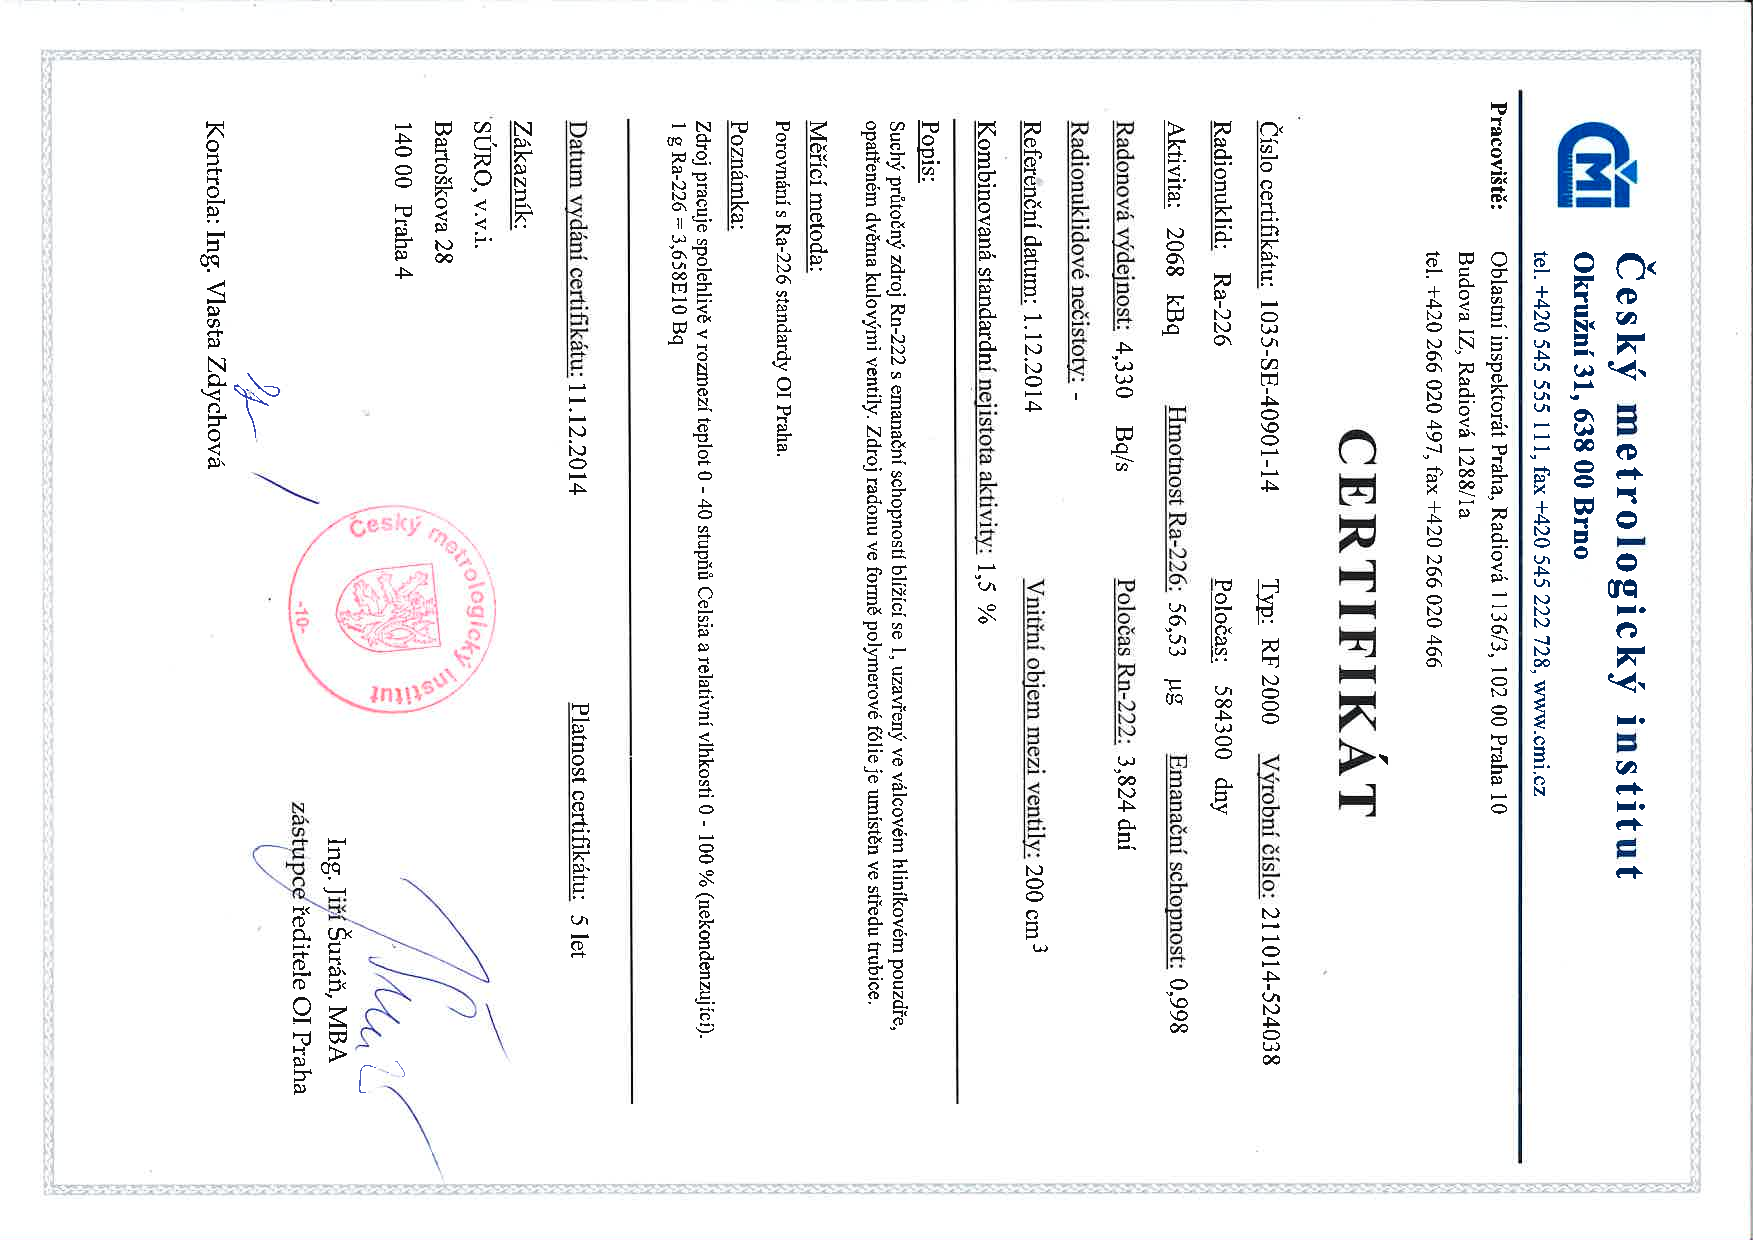
\includegraphics[page=1, angle=90, scale=0.7]{zdroje.pdf}
\newpage
\includegraphics[page=2, angle=90, scale=0.7]{zdroje.pdf}
%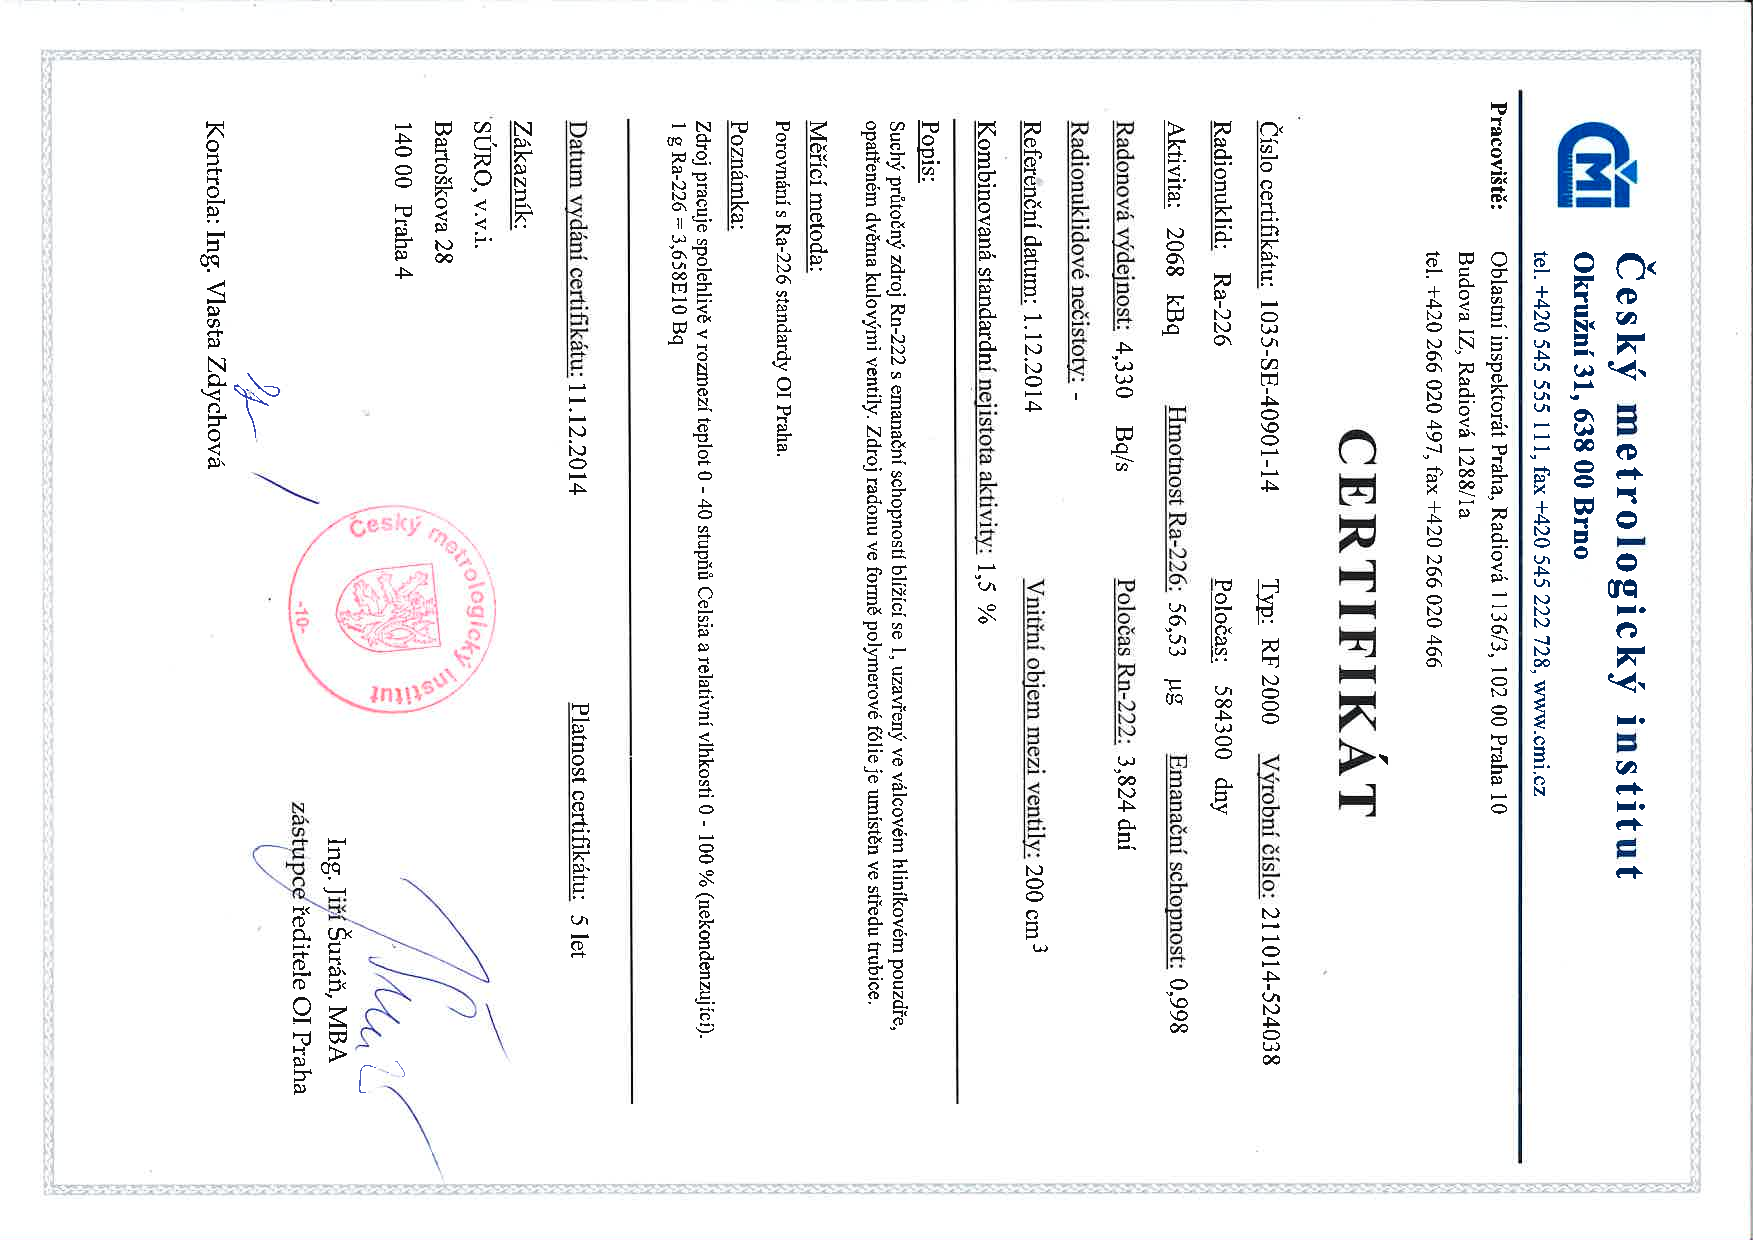
\includepdf[page=1, angle=90, scale=0.5]{zdroje.pdf}

\chapter{Přílohy k objektu Skála 75, okr. Havlíčkův Brod}\label{navesti:priloha_skala75}

\section{Fotografie objektu}

\begin{figure}[H]
    \centering
    \includegraphics[width=.6\textwidth]{skala75/humpolec_chata.jpg}
    \caption{Fotografie objektu z přední strany.}
    \label{fig:skala75}
\end{figure}

%\section{Naměřené vývoje OAR, teplot a relativní vlhkosti vzduchu}

%\begin{figure}[H]
    %\centering
    %%\includegraphics[height=0.8\textwidth, angle=-90, origin=c]{skala75/a1.png}
    %\includegraphics[width=1.1\textwidth]{skala75/a1.png}
    %\caption{Data z TERA sondy č. 8, která byla umístěna ve sklepě.}
    %\label{fig:skala75_a1}
%\end{figure}
%\begin{figure}[H]
    %\centering
    %%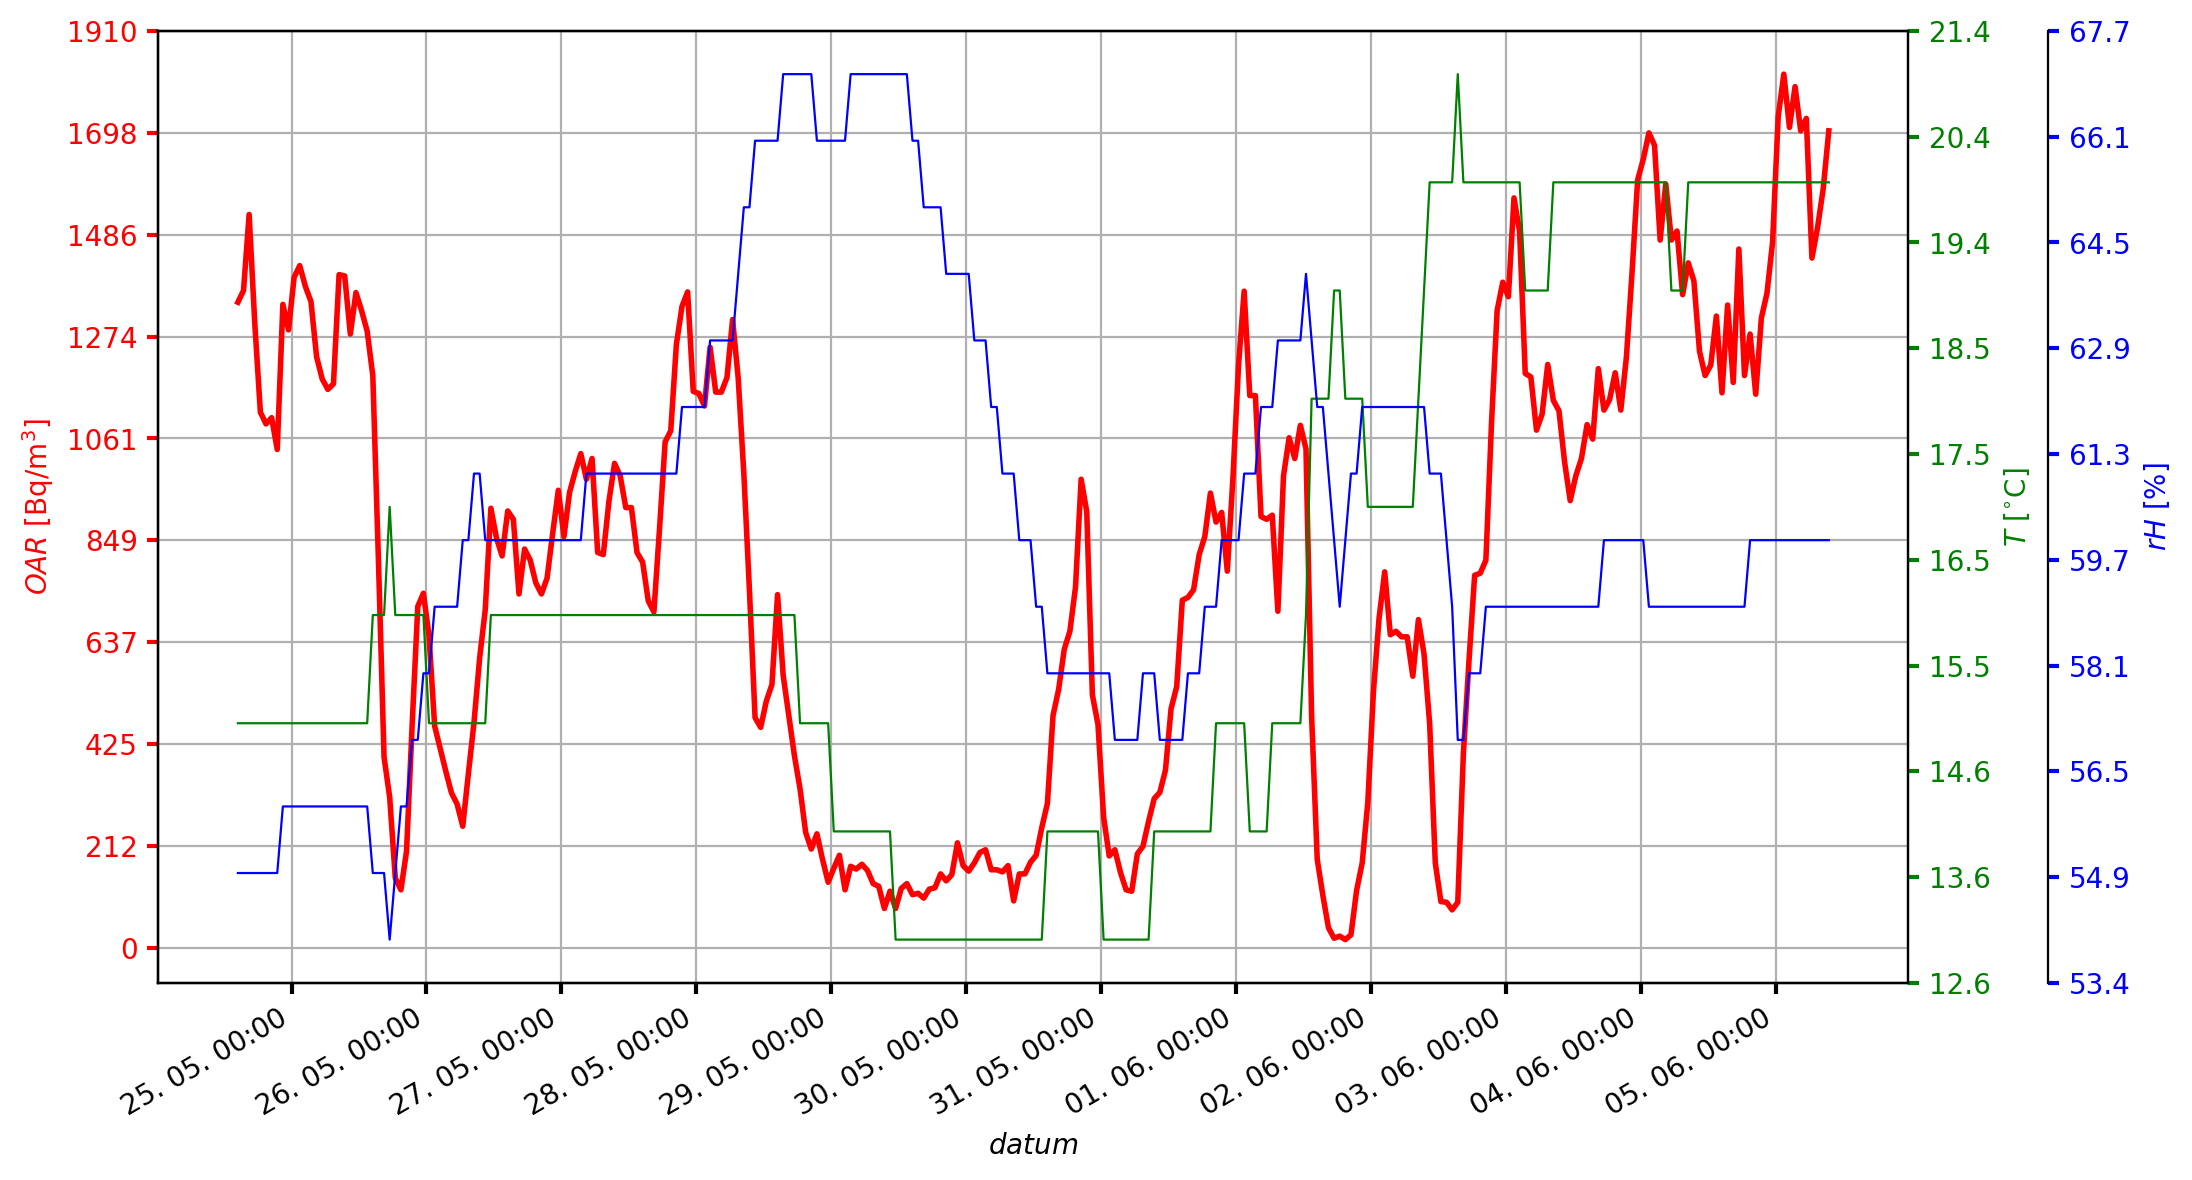
\includegraphics[height=0.8\textwidth, angle=-90, origin=c]{skala75/a2_1.png}
    %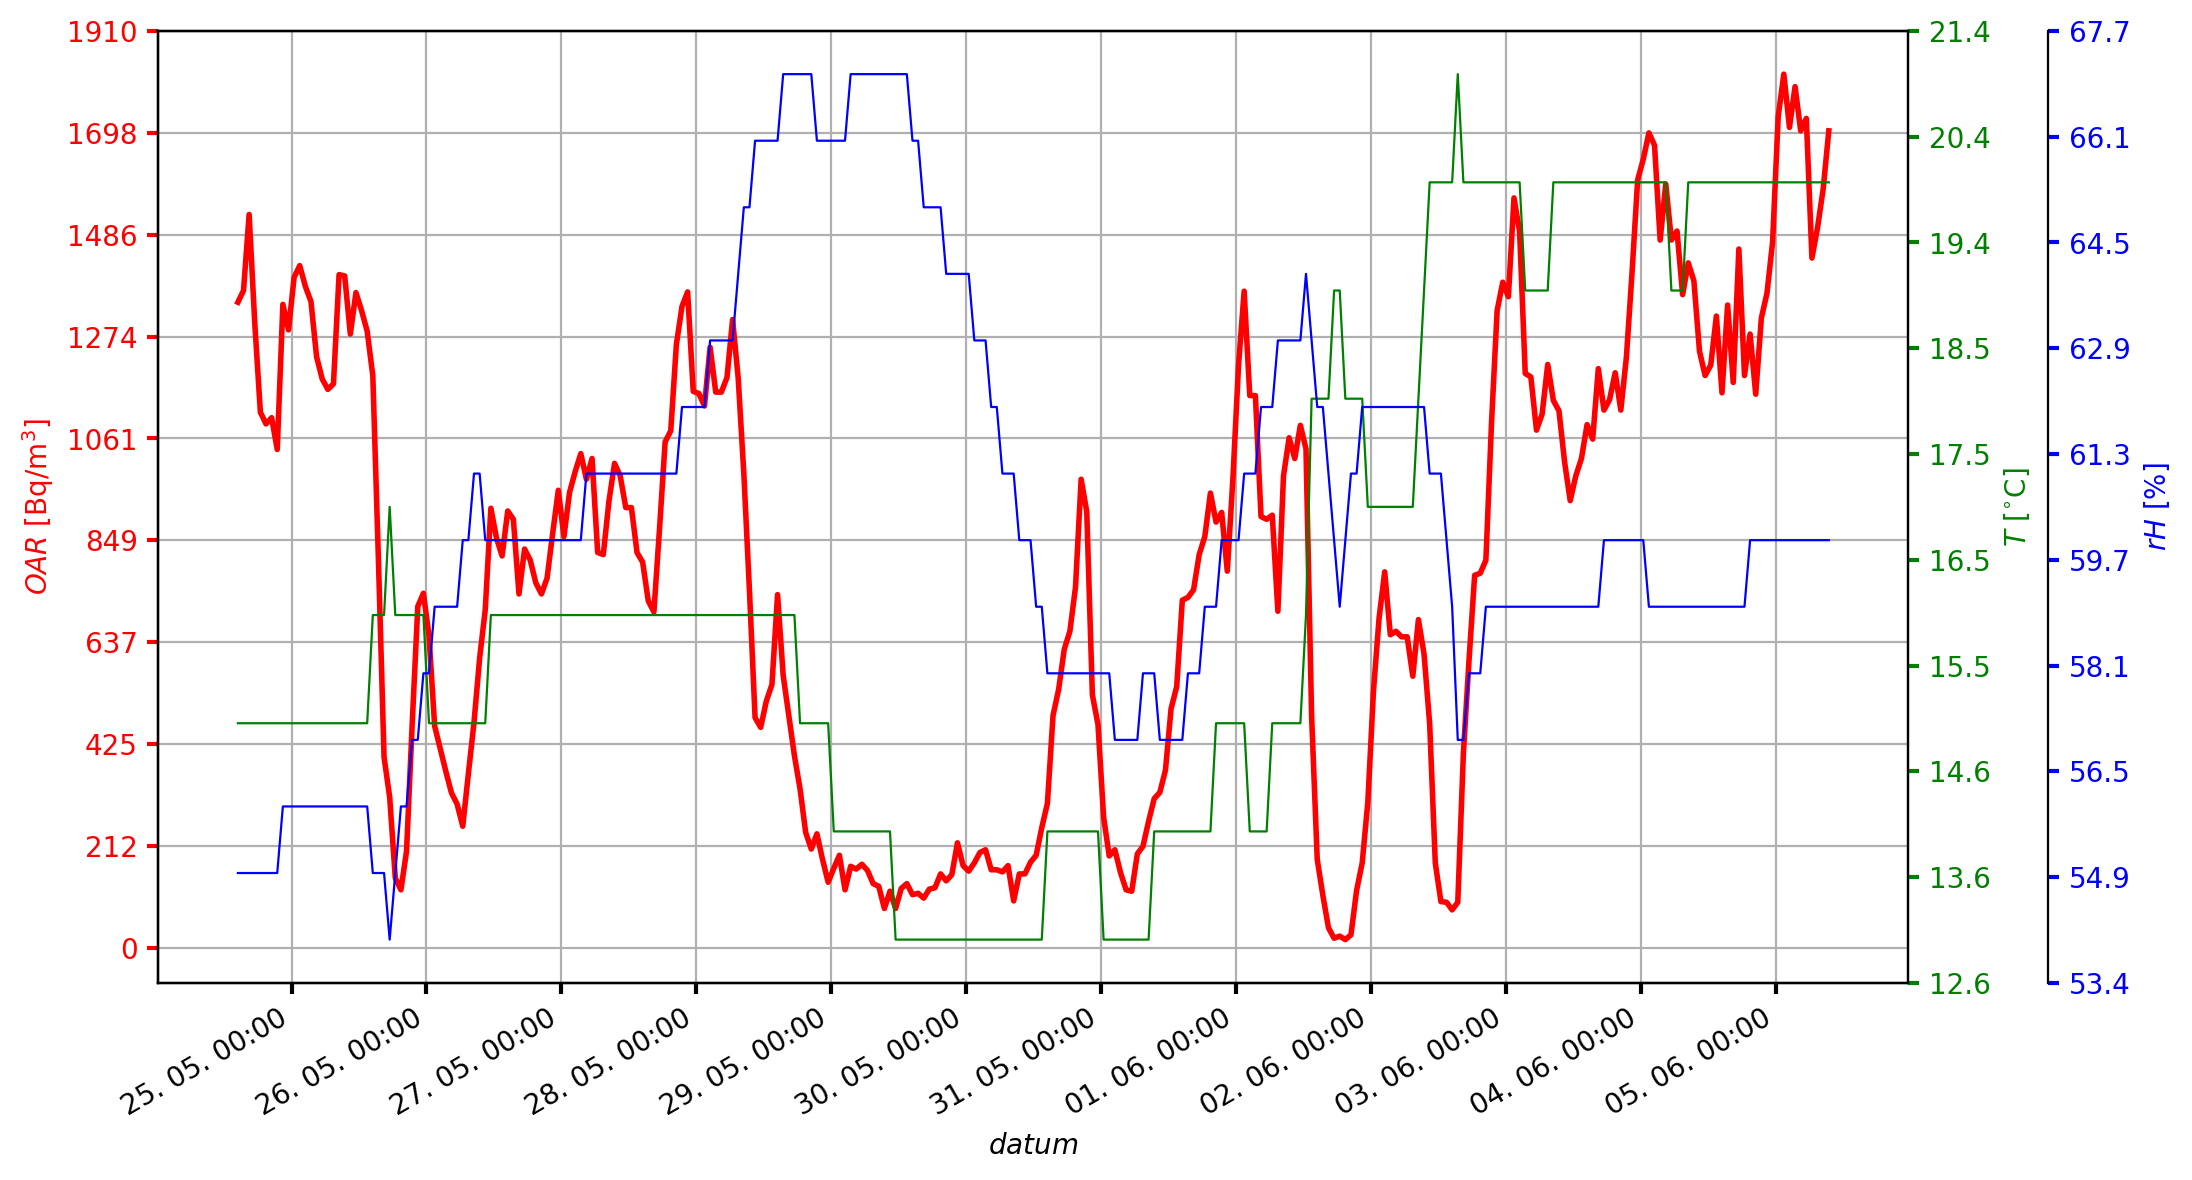
\includegraphics[width=1.1\textwidth]{skala75/a2_1.png}
    %\caption{Data z TERA sondy č. 10, která byla umístěna v přízemí v kuchyni.}
    %\label{fig:skala75_a2_1}
%\end{figure}
%\begin{figure}[H]
    %\centering
    %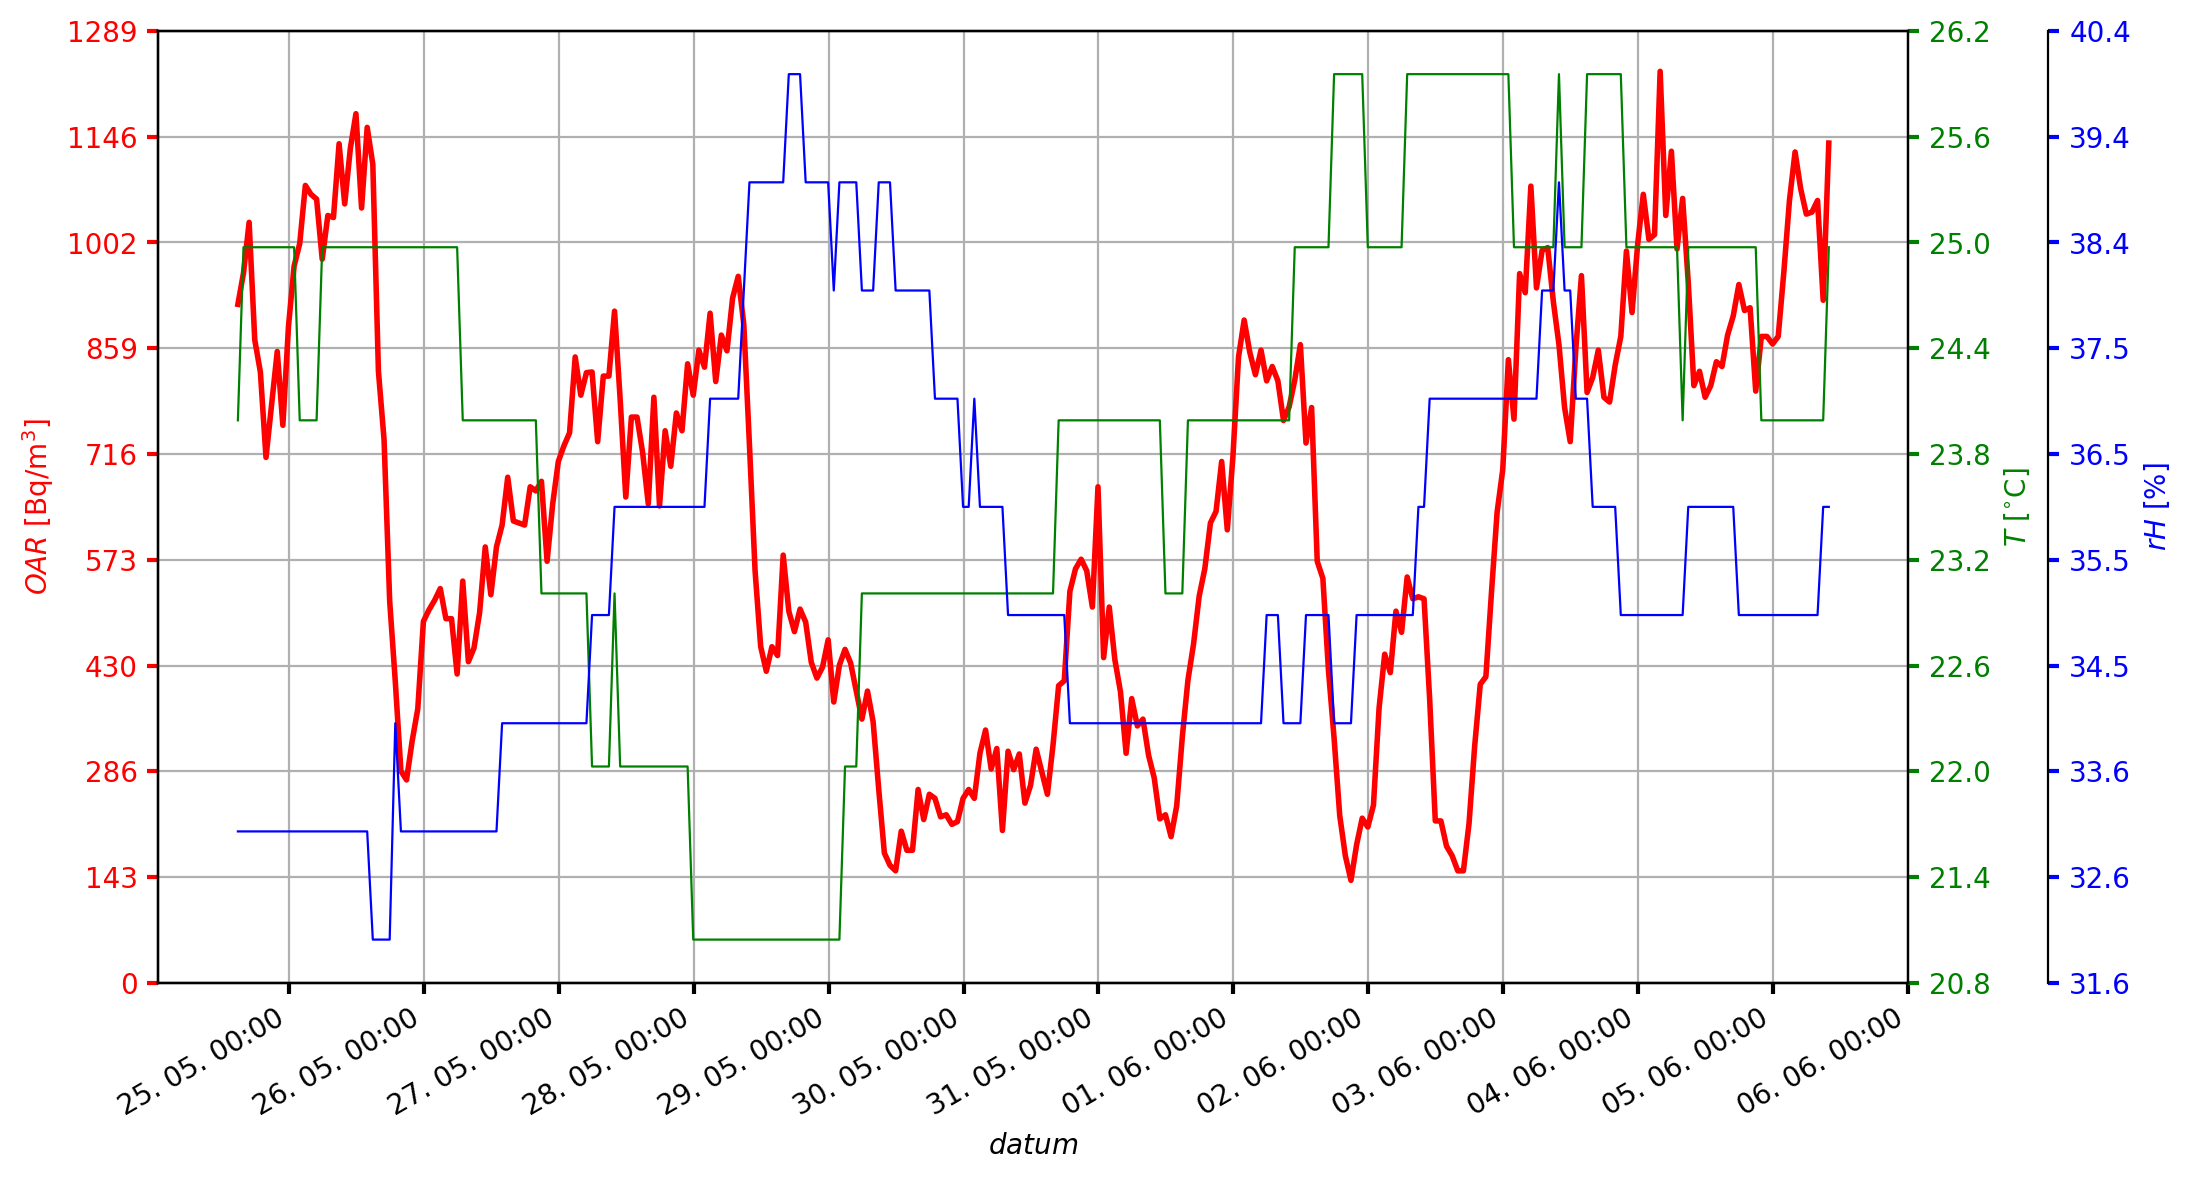
\includegraphics[width=1.1\textwidth]{skala75/a2_2.png}
    %\caption{Data z TERA sondy č. 112, která byla umístěna v přízemí v ložnici.}
    %\label{fig:skala75_a2_2}
%\end{figure}
%\begin{figure}[H]
    %\centering
    %\includegraphics[width=1.1\textwidth]{skala75/a3.png}
    %\caption{Data z TERA sondy č. 88, která byla umístěna v prvním patře.}
    %\label{fig:skala75_a3}
%\end{figure}

\section{Použitá měřidla}
\begin{itemize}
    \setlength\itemsep{0em}
	\item 14 vyvíječů (2x TMH, 2x TCE, 3x MDC, 3x MCH, 2x PCE, 2x PCH)
	\item 12 TD detektorů
	\item 4 CANARY monitory
	\item 4 TERA sondy
	\item 3 TESTO měřiče teploty a vlhkosti
	\item 2 zdroje radonu
\end{itemize}

\section{Naměřené OAR, objemy a teploty}

\begin{table}[H]
    \centering
    \caption{Objemy podlaží objektu, průměrné teploty naměřené v každém podlaží dataloggery testo 174H, odhadnuté atmosférické tlaky v každém podlaží a přiřazení číslování kompartmentů jednotlivým podlažím. Význam označení podlaží je vysvětlen v tab. \ref{tab:rovMer_podlazi}.}
    \label{tab:skala75_objemy}
    \begin{tabular}{lll}
\toprule
podlazi & $OAR$ [\si{Bq/m^3}] & $V$ [\si{m^3}] \\
\midrule
0 &           1094+/-55 &         40+/-8 \\
1 &            562+/-20 &        84+/-10 \\
2 &              51+/-2 &        97+/-15 \\
\bottomrule
\end{tabular}

\end{table}
\begin{figure}[H]
    \centering
    \includegraphics[width=1\textwidth]{skala75/OAR_dohromady.png}
    \caption{Vývoj OAR naměřený TERA sondami po aplikování kalibračních konstant (tab.~\ref{tab:dynMer_sondyB}). Pro další vyhodnocování byly OAR naměřené v přízemí v kuchyni a v ložnici zprůměrovány.}
    \label{fig:skala75_OAR_dohromady}
\end{figure}
\begin{figure}[H]
    \centering
    \includegraphics[width=1\textwidth]{skala75/OAR_CANARY.png}
    \caption{Vývoj OAR naměřený CANARY měřáky.}
    \label{fig:skala75_OAR_CANARY}
\end{figure}

\subsection{Průměrné hodnoty OAR}

\begin{table}[H]
    \centering
    \caption{Průměrné objemové koncentrace radonu naměřené TERA sondami umístěnými v uvedených podlažích. $\sigma_A$ je nejistota OAR typu A plynoucí ze statistického zpracování naměřených dat, $\sigma_B$ je nejistota OAR typu B plynoucí z ostatních zdrojů (statistika detekce, nejistota měřidla) a $\sigma$ je kombinovaná nejistota OAR. Při určování přísunů radonu v rovnovážném stavu byla použita pouze nejistota typu B, tj. $\sigma_B$. V posledním sloupci je průměrná citlivost TERA sond vypočtená z naměřených dat (tj. z naměřeného počtu impulzů a naměřeného OAR). Tato citlivost byla použita pro výpočet $\sigma_B$ (viz podkapitola~\ref{navesti:radon_TERAnejistota}).}
    \label{tab:skala75_OARprumerne}
    \begin{tabular}{llrrrrr}
\toprule
ID sondy&podlaží& OAR [\si{Bq/m^3}]& $\sigma_A$ & $\sigma_B$ &$\sigma$& $\overline{c}$ $\left[\si{\frac{imp}{hod}/\frac{Bq}{m^3}}\right]$\\ 
\midrule
8  &0 & 458 & 309 & 33 & 311&0,405\\
10 &1 & 789 & 485 & 43 & 487&0,433\\
112&1 & 633 & 282 & 37 & 284&0,464\\
88 &2 & 276 & 356 & 31 & 358&0,296\\
\bottomrule
    \end{tabular}
\end{table}

\begin{table}[H]
    \centering
    \caption{Průměrné OAR naměřené CANARY měřáky umístěnými v daných podlažích.}
    \label{tab:skala75_OARprumerne_CANARY}
    \begin{tabular}{llr}
        \toprule
        ID měřáku & podlaží & OAR [\si{Bq/m^3}]\\
        \midrule
        1 & 0 & $381\pm38$\\
        2 & 1 & $419\pm42$\\
        4 & 1 & $465\pm47$\\
        3 & 2 & $156\pm16$\\
        \bottomrule
    \end{tabular}
\end{table}

\section{Objemové průtoky vzduchu}

\begin{table}[H]
    \centering
    \caption{Přehled použitých indikačních plynů a umístění jejich vyvíječů v objektu. V posledním sloupci jsou celkové odpary plynů ze všech jim odpovídajících vyvíječů.}
    \label{tab:skala75_indikacniPlyny}
    \begin{tabular}{lrrrr}
\toprule
ozn. & podlaží& odpar [mg] &    $M$ [g/mol] &    $U$ $\left[\si{\frac{ng}{ppm\cdot min}}\right]$\\
\midrule
TMH & 0 &192,50 &  450,0 &  8,000 \\
TCE & 0 &193,55 &  130,4 &  1,000 \\
MCH & 1 &472,27 &  350,0 &  8,000 \\
MDC & 1 &497,27 &  400,0 &  8,000 \\
PCH & 2 &230,88 &  450,0 &  8,000 \\
PCE & 2 & 96,54 &  165,8 &  1,385 \\
\bottomrule
\end{tabular}

\end{table}
\begin{table}[H]
    \centering
    \caption{Odezvy TD detektorů $R$ na všechny použité indikační plyny ve všech zónách.}
    \label{tab:skala75_odezvyTD}
    \begin{tabular}{lrr}
\toprule
plyn & zóna & $R$ [\si{ng}]               \\
\midrule
MCH & 1 & $  36,0\pm2,3$\\
    & 2 & $395,8\pm16,6$\\
    & 3 & $  50,8\pm2,3$\\
MDC & 1 & $  34,5\pm1,2$\\
    & 2 & $ 304,9\pm7,1$\\
    & 3 & $  47,2\pm1,2$\\
TMH & 1 & $145,3\pm26,0$\\
    & 2 & $  37,5\pm3,9$\\
    & 3 & $  20,2\pm2,4$\\
PCH & 1 & $  20,7\pm2,4$\\
    & 2 & $  26,9\pm0,7$\\
    & 3 & $ 182,2\pm4,6$\\
TCE & 1 & $191,8\pm14,5$\\
    & 2 & $  32,2\pm1,4$\\
    & 3 & $  25,0\pm1,2$\\
PCE & 1 & $     0,0\pm0,0$\\
    & 2 & $   2,6\pm0,1$\\
    & 3 & $ 136,9\pm4,1$\\
\bottomrule
\end{tabular}

\end{table}

\begin{table}[H]
    \centering
    \caption{Objemové průtoky vzduchu v \si{m^3/hod} pro všechny kombinace aplikovaných indikačních plynů. $n$ je výměna vzduchu vypočtená ze vztahu~\eqref{eq:prutoky_n}, $[n]=\si{1/hod}$.}
    \label{tab:skala75_prutoky}
\begin{tabular}{l>{\raggedleft\arraybackslash}p{2.5cm}>{\raggedleft\arraybackslash}p{2.5cm}>{\raggedleft\arraybackslash}p{2.5cm}>{\raggedleft\arraybackslash}p{2.5cm}}
\toprule
{} & (TMH, MDC, PCE) & (TMH, MDC, PCH) & (TMH, MCH, PCE) & (TMH, MCH, PCH)\\ 
\midrule
$k_{12}$ &12,262$\pm$3,129 &  11,759$\pm$3,078 &  10,188$\pm$2,611 &   9,746$\pm$2,563 \\          
$k_{13}$ & 0,855$\pm$0,255 &   3,372$\pm$1,013 &   0,908$\pm$0,261 &   3,573$\pm$1,036 \\          
$k_{21}$ & 4,028$\pm$0,940 &   3,507$\pm$0,847 &   3,220$\pm$0,776 &   2,780$\pm$0,700 \\          
$k_{23}$ & 1,240$\pm$0,183 &   4,889$\pm$0,724 &   1,025$\pm$0,161 &   4,031$\pm$0,635 \\          
$k_{31}$ &-0,076$\pm$0,020 &   3,524$\pm$0,958 &  -0,061$\pm$0,016 &   3,611$\pm$0,968 \\          
$k_{32}$ & 0,931$\pm$0,137 &   5,967$\pm$0,967 &   0,774$\pm$0,117 &   4,945$\pm$0,820 \\          
&&&&\\
$k_{1_E}$&21,425$\pm$5,271 &  19,770$\pm$5,057 &  23,244$\pm$5,443 &  21,411$\pm$5,208 \\          
$k_{2_E}$&44,024$\pm$4,853 &  41,624$\pm$4,833 &  36,712$\pm$4,240 &  34,644$\pm$4,195 \\          
$k_{3_E}$& 7,712$\pm$0,849 &  24,294$\pm$3,199 &   7,850$\pm$0,853 &  25,127$\pm$3,209 \\          
$k_{1_I}$&30,590$\pm$6,206 &  27,869$\pm$6,140 &  31,181$\pm$6,093 &  28,339$\pm$6,017 \\          
$k_{2_I}$&36,099$\pm$5,855 &  32,294$\pm$5,917 &  29,994$\pm$5,043 &  26,764$\pm$5,073 \\          
$k_{3_I}$& 6,472$\pm$0,916 &  25,525$\pm$3,693 &   6,630$\pm$0,914 &  26,079$\pm$3,658 \\          
\midrule                                                                              
$n$      & 0,310$\pm$0,038 &   0,363$\pm$0,042 &   0,287$\pm$0,036 &   0,344$\pm$0,041 \\
\bottomrule
\end{tabular}
\vspace{0.5cm}

\begin{tabular}{l>{\raggedleft\arraybackslash}p{2.5cm}>{\raggedleft\arraybackslash}p{2.5cm}>{\raggedleft\arraybackslash}p{2.5cm}>{\raggedleft\arraybackslash}p{2.5cm}}
    \toprule
    {} & (TCE, MDC, PCE) & (TCE, MDC, PCH) & (TCE, MCH, PCE) & (TCE, MCH, PCH) \\
    \midrule
$k_{12}$ & 7,859$\pm$1,288 &   7,286$\pm$1,238 &   6,544$\pm$1,094 &   6,050$\pm$1,047 \\
$k_{13}$ & 0,893$\pm$0,159 &   3,523$\pm$0,631 &   0,927$\pm$0,162 &   3,647$\pm$0,641 \\
$k_{21}$ & 1,309$\pm$0,211 &   1,140$\pm$0,195 &   1,049$\pm$0,182 &   0,906$\pm$0,169 \\
$k_{23}$ & 1,235$\pm$0,180 &   4,874$\pm$0,715 &   1,023$\pm$0,159 &   4,025$\pm$0,628 \\
$k_{31}$ &-0,025$\pm$0,005 &   1,146$\pm$0,243 &  -0,020$\pm$0,004 &   1,176$\pm$0,245 \\
$k_{32}$ & 0,922$\pm$0,136 &   6,419$\pm$0,960 &   0,767$\pm$0,116 &   5,330$\pm$0,817 \\
&&&&\\
$k_{1_E}$& 2,474$\pm$1,325 &   0,539$\pm$1,320 &   3,713$\pm$1,256 &   1,616$\pm$1,248 \\
$k_{2_E}$&46,234$\pm$4,862 &  43,556$\pm$4,848 &  38,543$\pm$4,268 &  36,229$\pm$4,226 \\
$k_{3_E}$& 7,670$\pm$0,848 &  26,236$\pm$3,237 &   7,815$\pm$0,852 &  27,185$\pm$3,242 \\
$k_{1_I}$& 9,941$\pm$1,867 &   9,061$\pm$1,942 &  10,155$\pm$1,683 &   9,231$\pm$1,776 \\
$k_{2_I}$&39,997$\pm$5,039 &  35,866$\pm$5,149 &  33,303$\pm$4,414 &  29,780$\pm$4,477 \\
$k_{3_I}$& 6,439$\pm$0,891 &  25,404$\pm$3,517 &   6,613$\pm$0,889 &  26,019$\pm$3,470 \\
\midrule                                                                                 
$n$      & 0,239$\pm$0,028 &   0,298$\pm$0,034 &   0,212$\pm$0,025 &   0,275$\pm$0,031 \\
\bottomrule
\end{tabular}
\end{table}

\section{Přísuny radonu - grafy a statistiky}\label{navesti:priloha_skala75_prisuny}
V tomto oddíle jsou uvedeny časové vývoje $Q_i(t)$ z naměřených časových vývojů OAR TERA sondami pro všechny kombinace použitých indikačních plynů.
\begin{figure}[H]
    \centering
    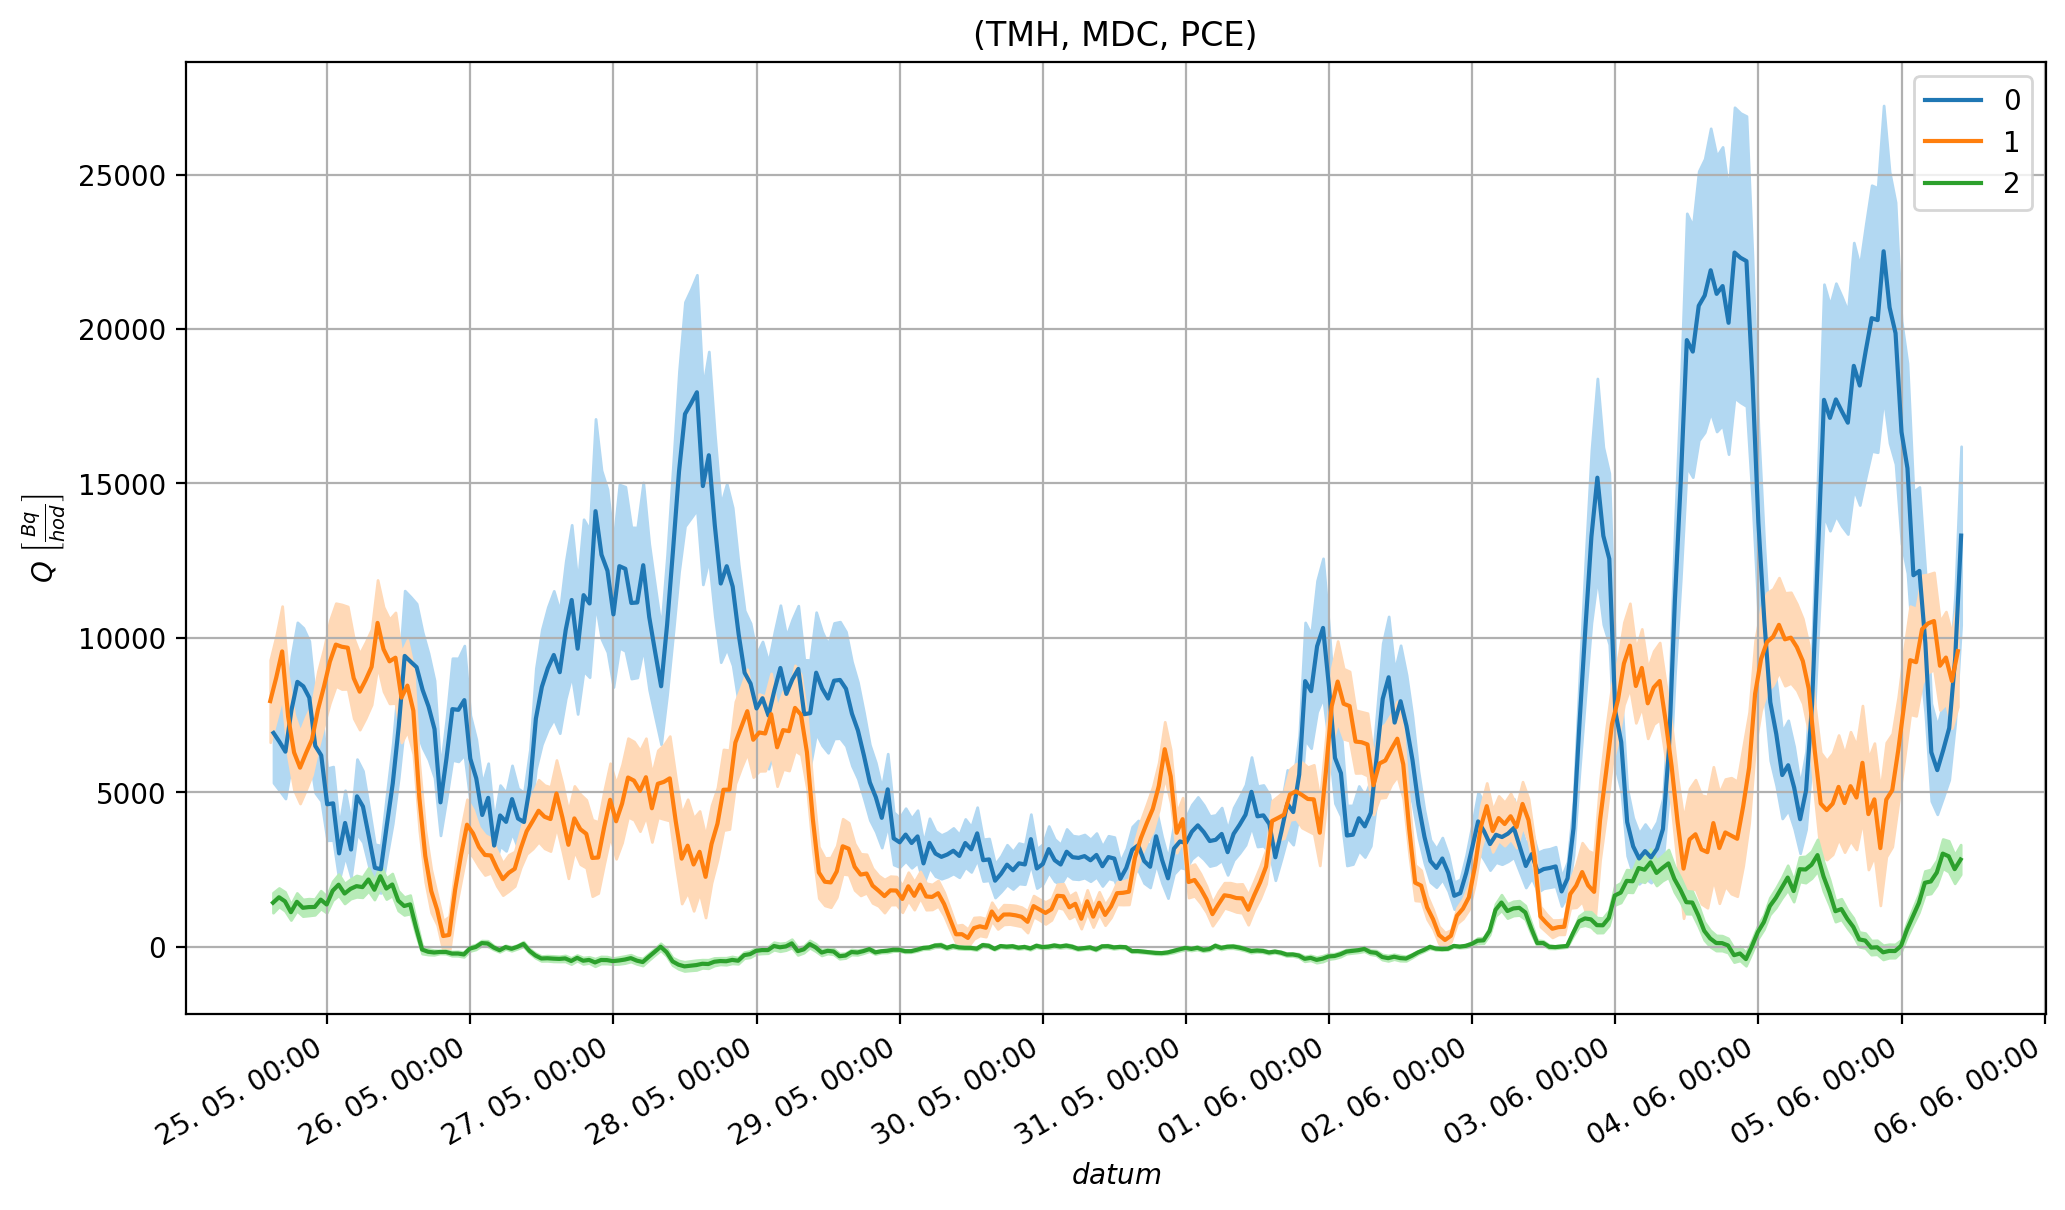
\includegraphics[width=\textwidth]{skala75/prisuny1.png}
    \caption{Určený časový vývoj přísunů radonu do jednotlivých podlaží. Nad obrázkem je uvedena kombinace tří použitých indikačních plynů. Oblasti označené zesvětlenou barvou značí nejistotu přísunů radonu při faktoru pokrytí $k=1$.}
    \label{fig:skala75_prisuny1}
\end{figure}
\begin{table}[H]
    \centering
    \caption{Statistiky vypočítaných přísunů radonu $Q$ do jednotlivých podlaží při stejné kombinaci použitých plynů jako v obr. nad touto tabulkou.}
    \label{tab:skala75_prisuny1}
    \begin{tabular}{lrrr}
\toprule
{} &  $Q_0$ $\left[\si{\frac{Bq}{m^3\cdot hod}}\right]$ &  $Q_1$ $\left[\si{\frac{Bq}{m^3\cdot hod}}\right]$ &  $Q_2$ $\left[\si{\frac{Bq}{m^3\cdot hod}}\right]$ \\
\midrule
count &                                                284 &                                                284 &                                                284 \\
mean  &                                                337 &                                                237 &                                                 19 \\
std   &                                                270 &                                                157 &                                                 84 \\
min   &                                                 15 &                                                -85 &                                               -269 \\
25%   &                                                137 &                                                102 &                                                -19 \\
50%   &                                                222 &                                                237 &                                                 -2 \\
75%   &                                                449 &                                                352 &                                                 29 \\
max   &                                               1161 &                                                891 &                                                371 \\
\bottomrule
\end{tabular}

\end{table}

\begin{figure}[H]
    \centering
    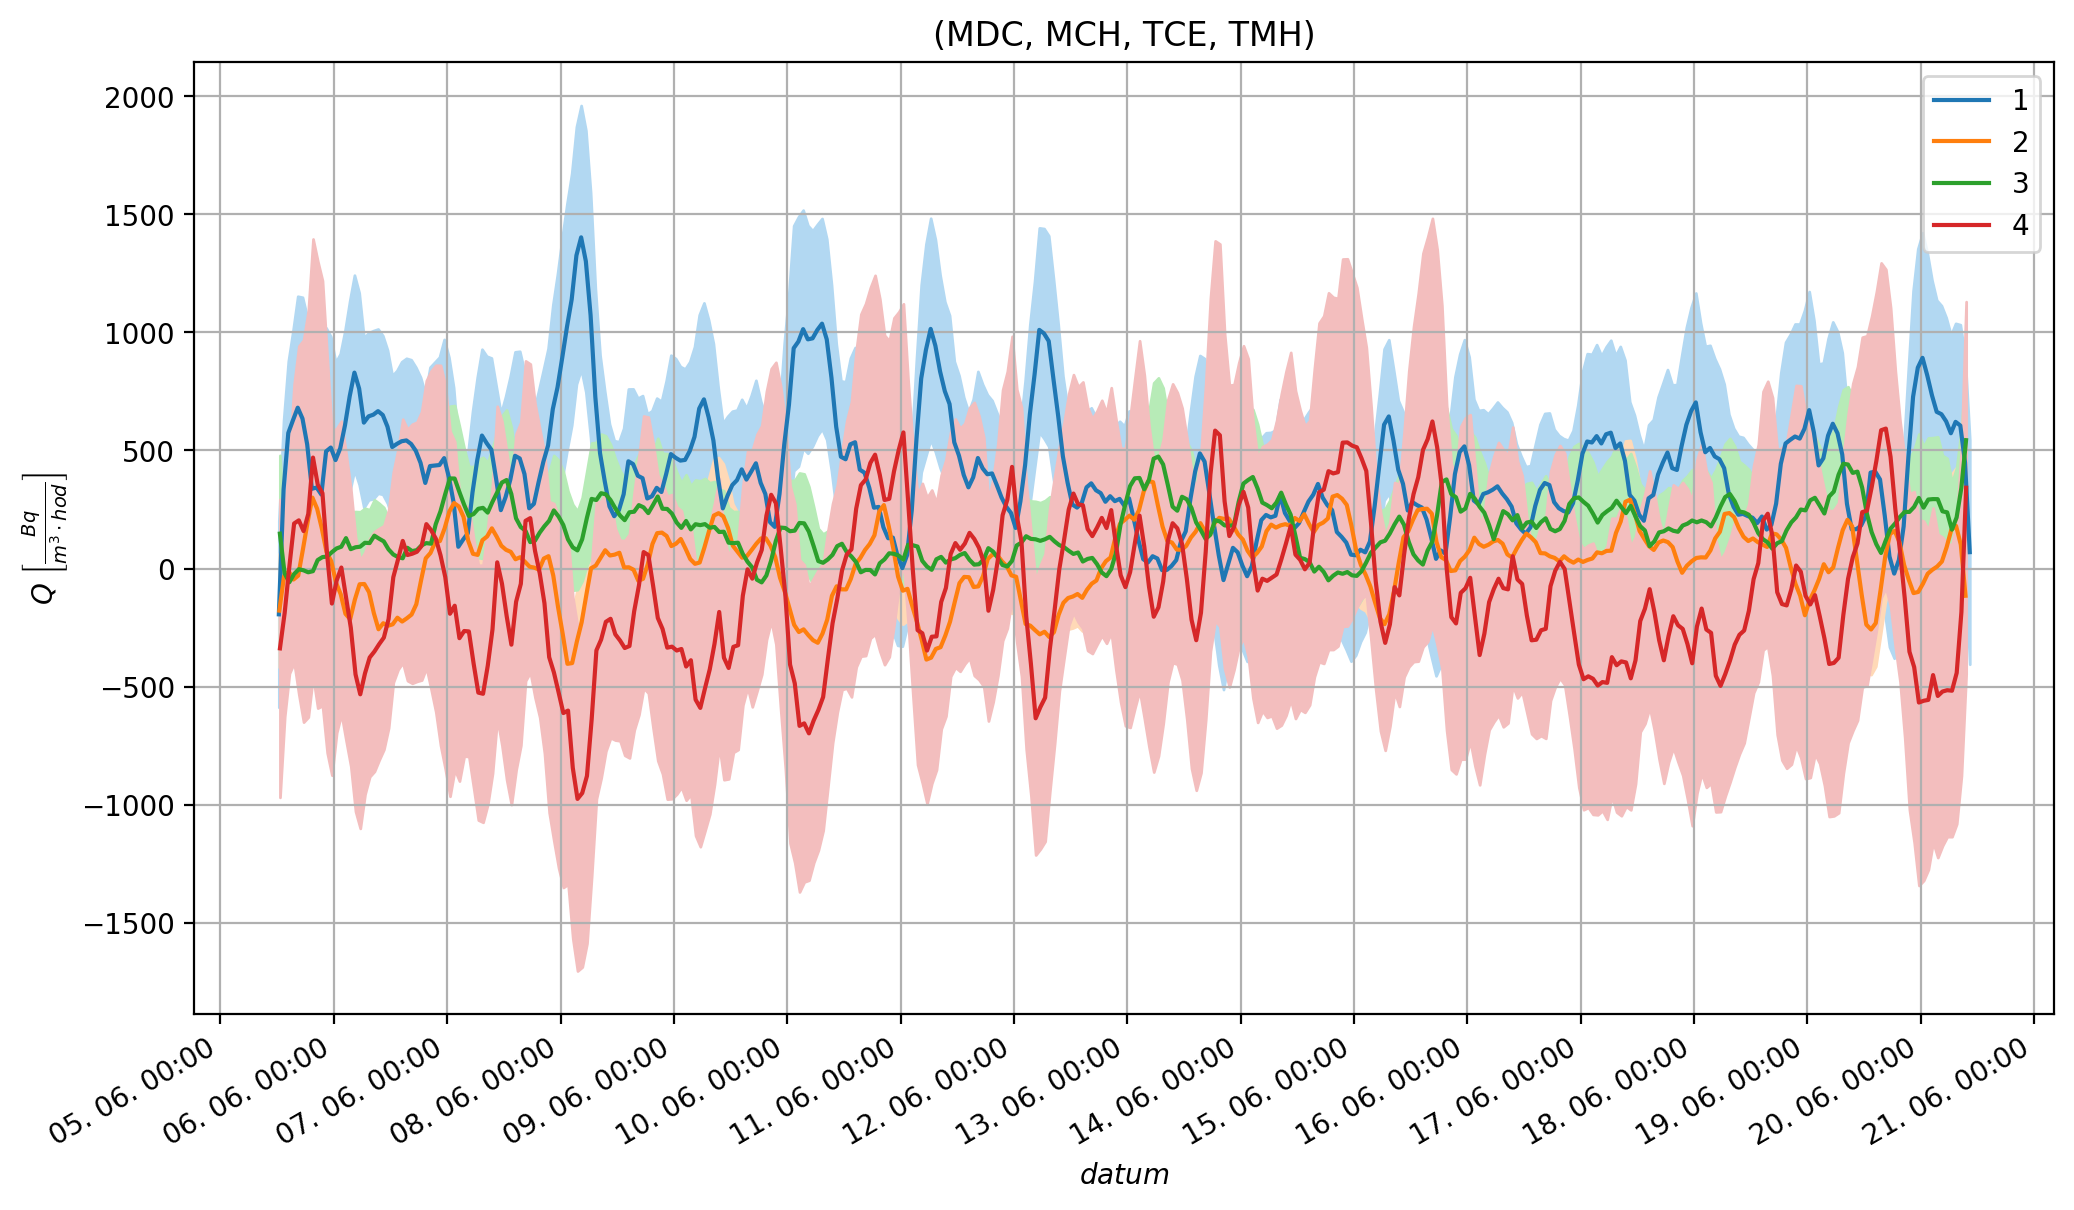
\includegraphics[width=\textwidth]{skala75/prisuny2.png}
    \caption{Určený časový vývoj přísunů radonu do jednotlivých podlaží. Nad obrázkem je uvedena kombinace tří použitých indikačních plynů. Oblasti označené zesvětlenou barvou značí nejistotu přísunů radonu při faktoru pokrytí $k=1$.}
    \label{fig:skala75_prisuny2}
\end{figure}
\begin{table}[H]
    \centering
    \caption{Statistiky vypočítaných přísunů radonu $Q$ do jednotlivých podlaží při stejné kombinaci použitých indikačních plynů jako v obr. nad touto tabulkou.}
    \label{tab:skala75_prisuny2}
    \begin{tabular}{lrrr}
\toprule
{} &  $Q_0$ $\left[\si{\frac{Bq}{hod}}\right]$ &  $Q_1$ $\left[\si{\frac{Bq}{hod}}\right]$ &  $Q_2$ $\left[\si{\frac{Bq}{hod}}\right]$ \\
\midrule
count &                                       284 &                                       284 &                                       284 \\
mean  &                                     12509 &                                     29052 &                                      4320 \\
%std   &                                     10164 &                                     15971 &                                     10993 \\
min   &                                     -1305 &                                      2758 &                                     -7217 \\
25\%   &                                      5053 &                                     13800 &                                     -2574 \\
50\%   &                                      8450 &                                     29570 &                                      -410 \\
75\%   &                                     16517 &                                     41212 &                                     10192 \\
max   &                                     42325 &                                     61230 &                                     36875 \\
\bottomrule
\end{tabular}

\end{table}

\begin{figure}[H]
    \centering
    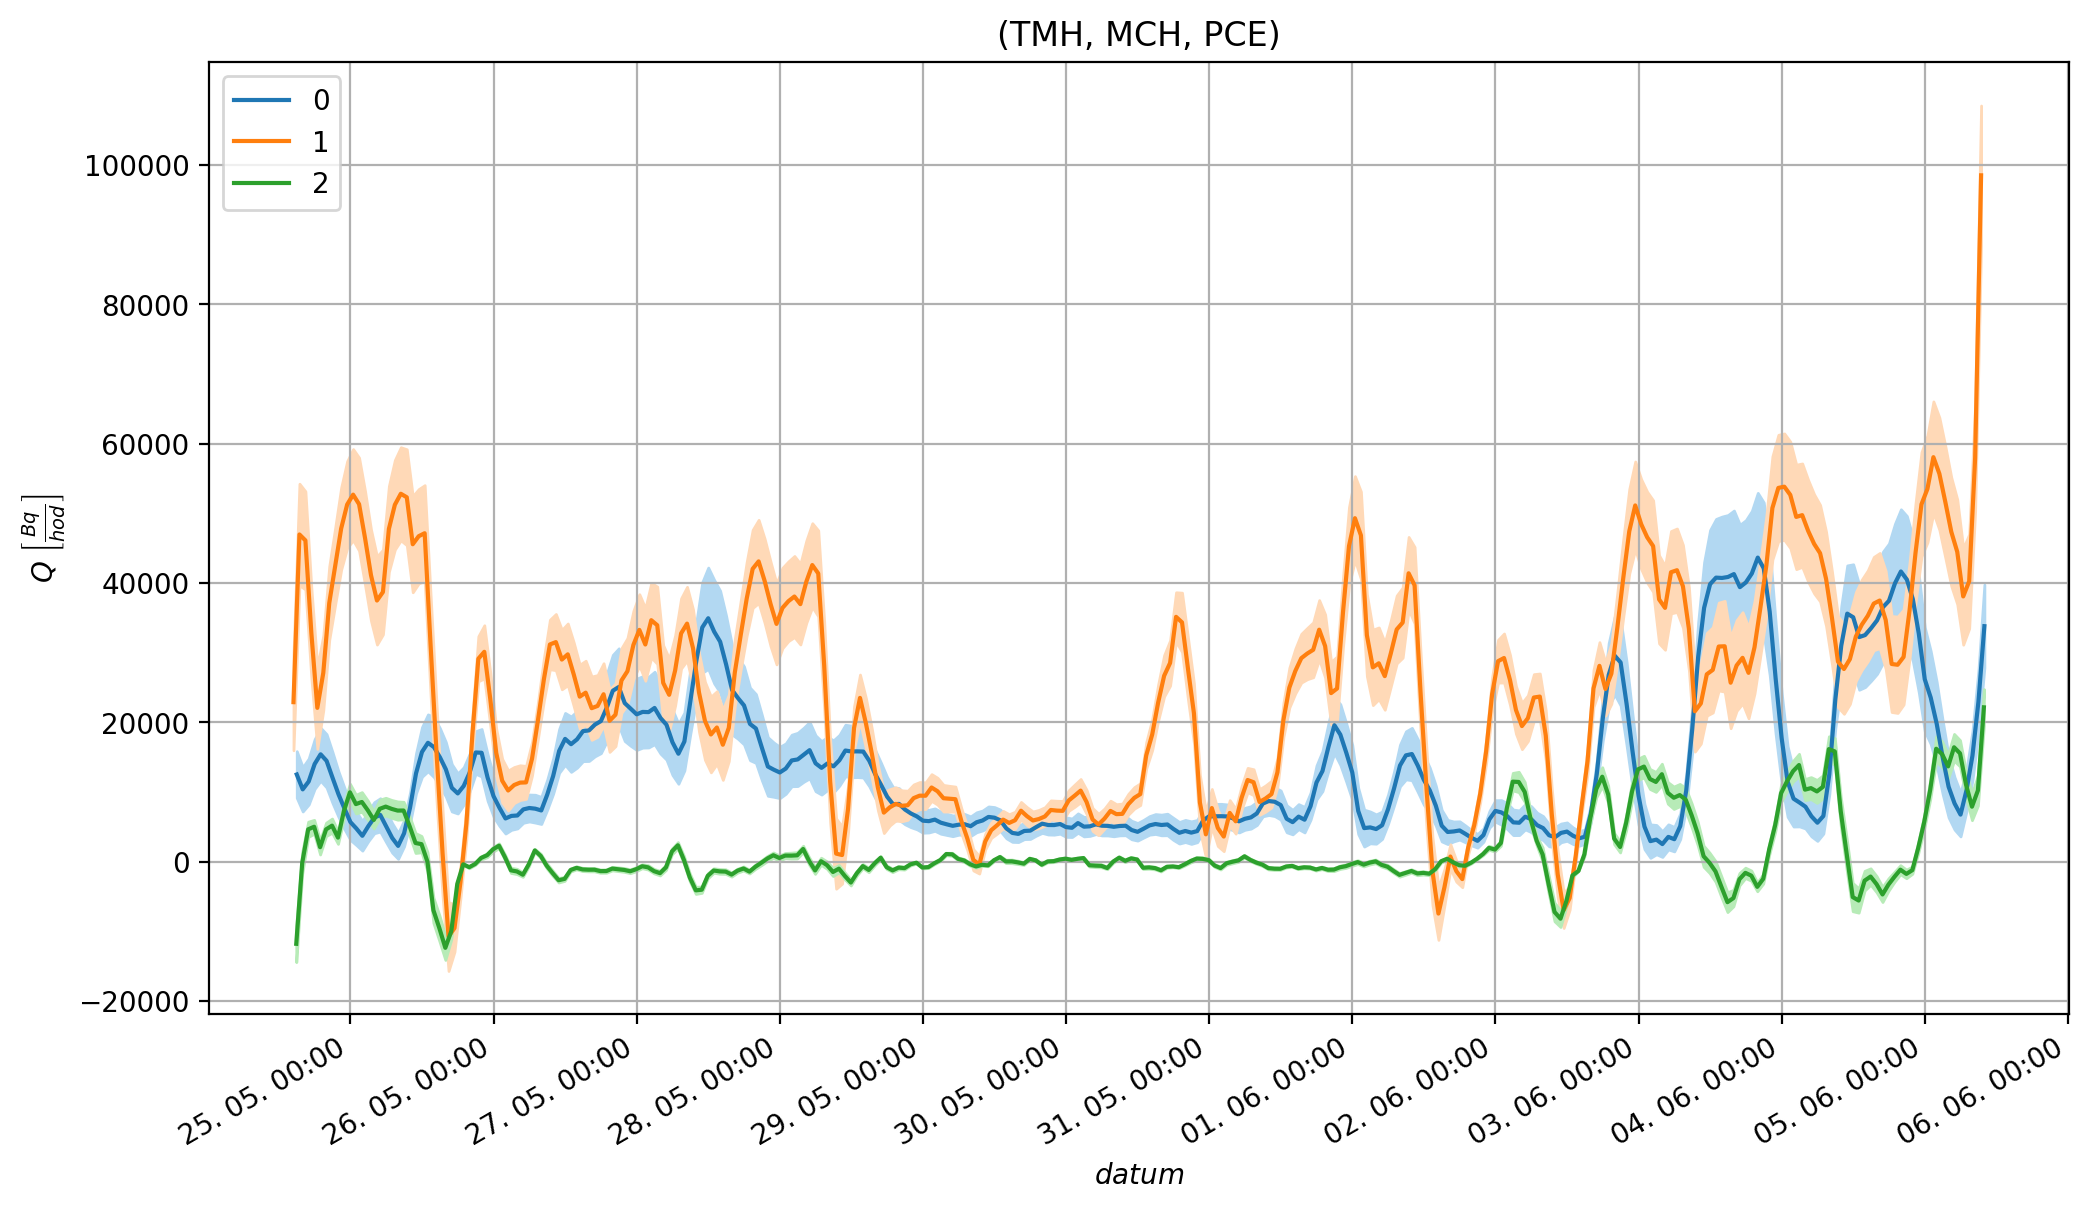
\includegraphics[width=\textwidth]{skala75/prisuny3.png}
    \caption{Určený časový vývoj přísunů radonu do jednotlivých podlaží. Nad obrázkem je uvedena kombinace tří použitých indikačních plynů. Oblasti označené zesvětlenou barvou značí nejistotu přísunů radonu při faktoru pokrytí $k=1$.}
    \label{fig:skala75_prisuny3}
\end{figure}
\begin{table}[H]
    \centering
    \caption{Statistiky vypočítaných přísunů radonu $Q$ do jednotlivých podlaží při stejné kombinaci použitých indikačních plynů jako v obr. nad touto tabulkou.}
    \label{tab:skala75_prisuny3}
    \begin{tabular}{lrrr}
\toprule
{} &  $Q_0$ $\left[\si{\frac{Bq}{hod}}\right]$ &  $Q_1$ $\left[\si{\frac{Bq}{hod}}\right]$ &  $Q_2$ $\left[\si{\frac{Bq}{hod}}\right]$ \\
\midrule
count &                                       284 &                                       284 &                                       284 \\
mean  &                                     13429 &                                     24771 &                                      1333 \\
std   &                                     10114 &                                     14050 &                                      2973 \\
min   &                                      2390 &                                      2315 &                                     -1709 \\
25%   &                                      5647 &                                     11702 &                                      -535 \\
50%   &                                      9781 &                                     24454 &                                       -12 \\
75%   &                                     17323 &                                     35419 &                                      2907 \\
max   &                                     42770 &                                     53869 &                                     10103 \\
\bottomrule
\end{tabular}

\end{table}

\begin{figure}[H]
    \centering
    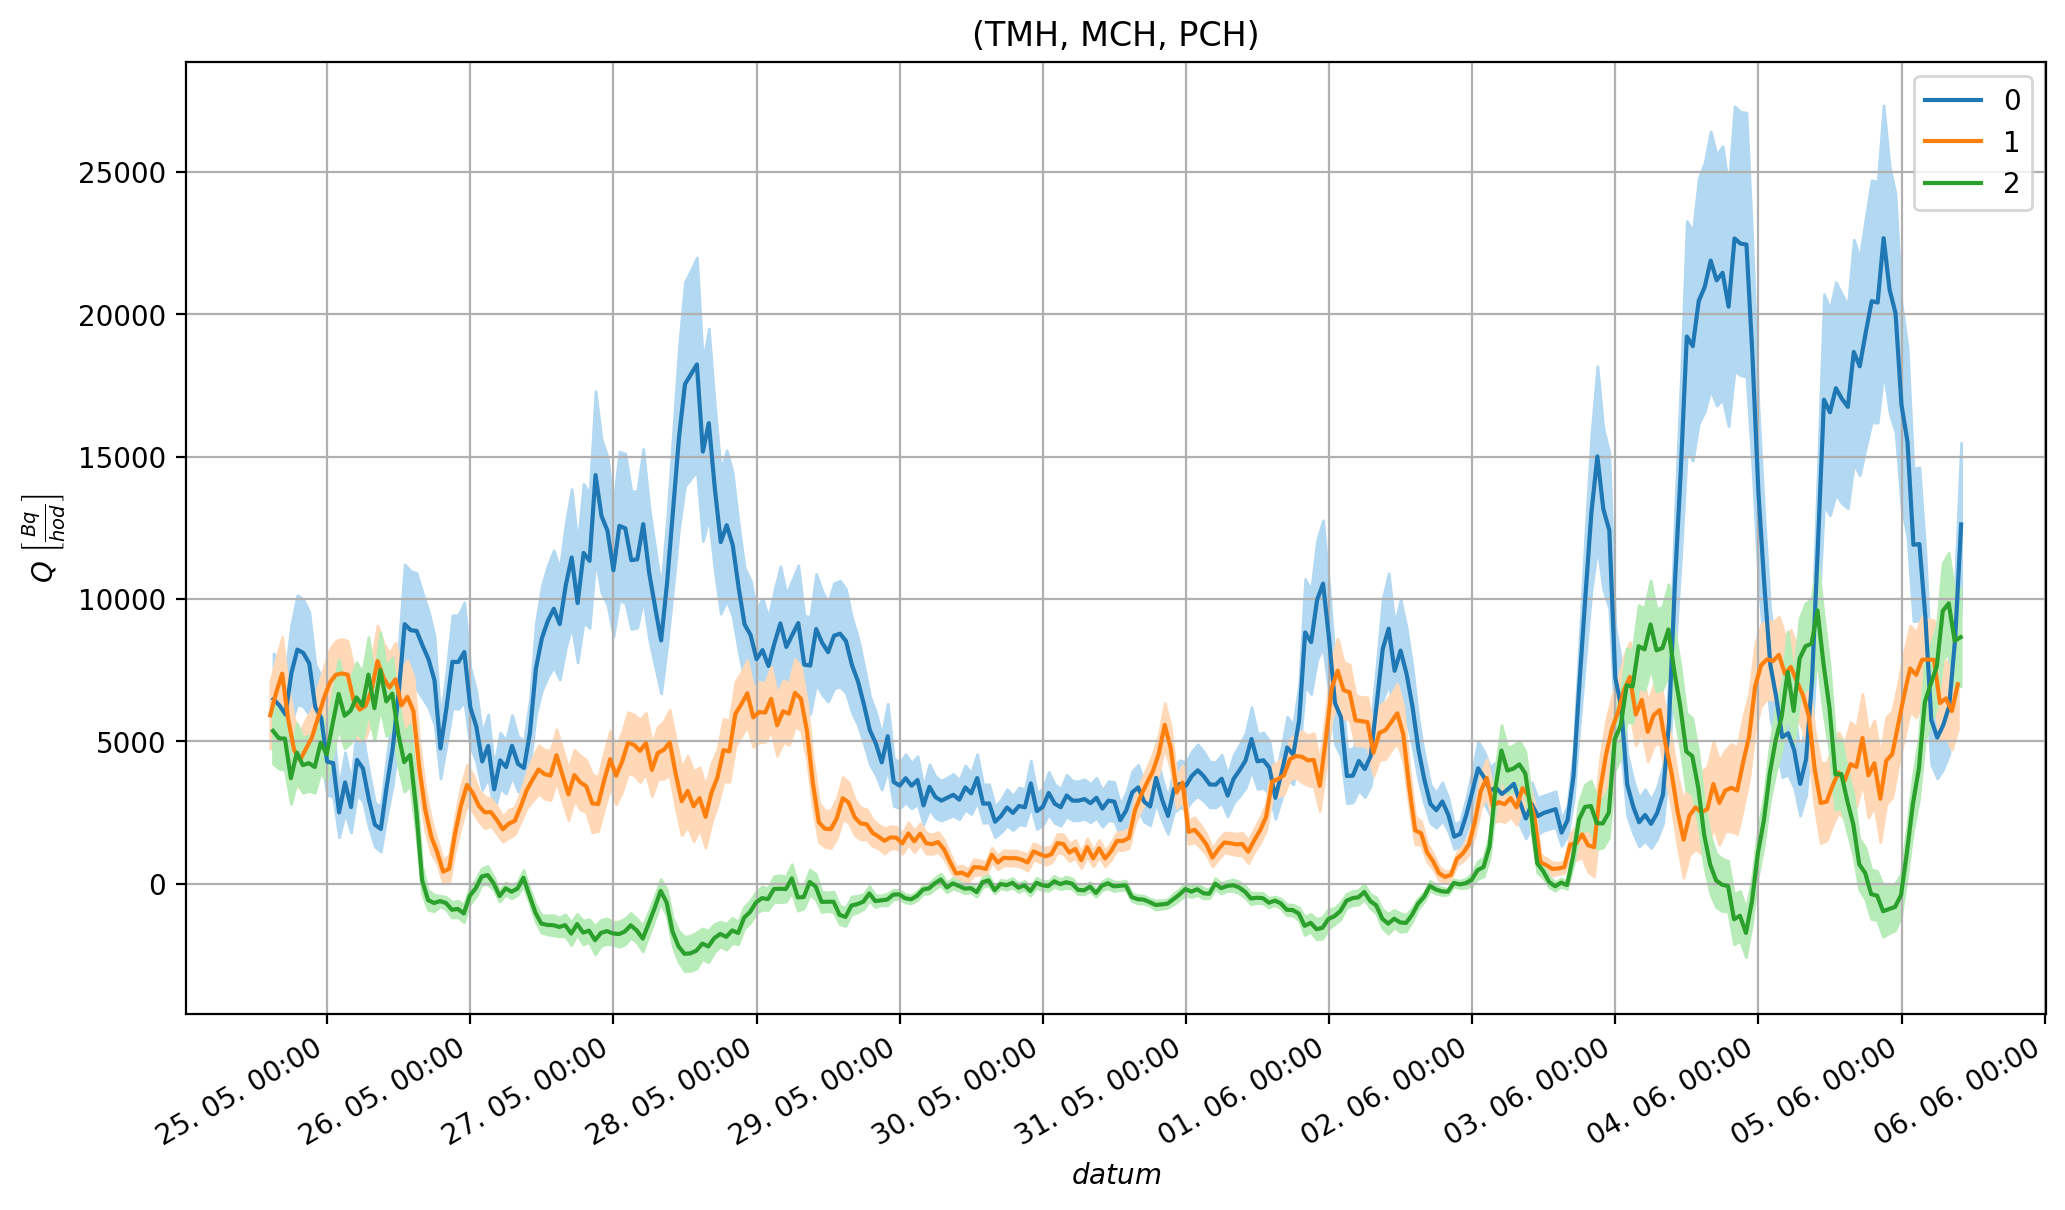
\includegraphics[width=\textwidth]{skala75/prisuny4.png}
    \caption{Určený časový vývoj přísunů radonu do jednotlivých podlaží. Nad obrázkem je uvedena kombinace tří použitých indikačních plynů. Oblasti označené zesvětlenou barvou značí nejistotu přísunů radonu při faktoru pokrytí $k=1$.}
    \label{fig:skala75_prisuny4}
\end{figure}
\begin{table}[H]
    \centering
    \caption{Statistiky vypočítaných přísunů radonu $Q$ do jednotlivých podlaží při stejné kombinaci použitých indikačních plynů jako v obr. nad touto tabulkou.}
    \label{tab:skala75_prisuny4}
    \begin{tabular}{lrrr}
\toprule
{} &  $Q_0$ $\left[\si{\frac{Bq}{hod}}\right]$ &  $Q_1$ $\left[\si{\frac{Bq}{hod}}\right]$ &  $Q_2$ $\left[\si{\frac{Bq}{hod}}\right]$ \\
\midrule
count &                                       284 &                                       284 &                                       284 \\
mean  &                                     12921 &                                     24194 &                                      4807 \\
%std   &                                     10215 &                                     13297 &                                     11131 \\
min   &                                      -501 &                                      2305 &                                     -6720 \\
25\%   &                                      5361 &                                     11493 &                                     -2236 \\
50\%   &                                      8950 &                                     24629 &                                      -191 \\
75\%   &                                     17045 &                                     34319 &                                     10881 \\
max   &                                     42783 &                                     50985 &                                     37529 \\
\bottomrule
\end{tabular}

\end{table}

\begin{figure}[H]
    \centering
    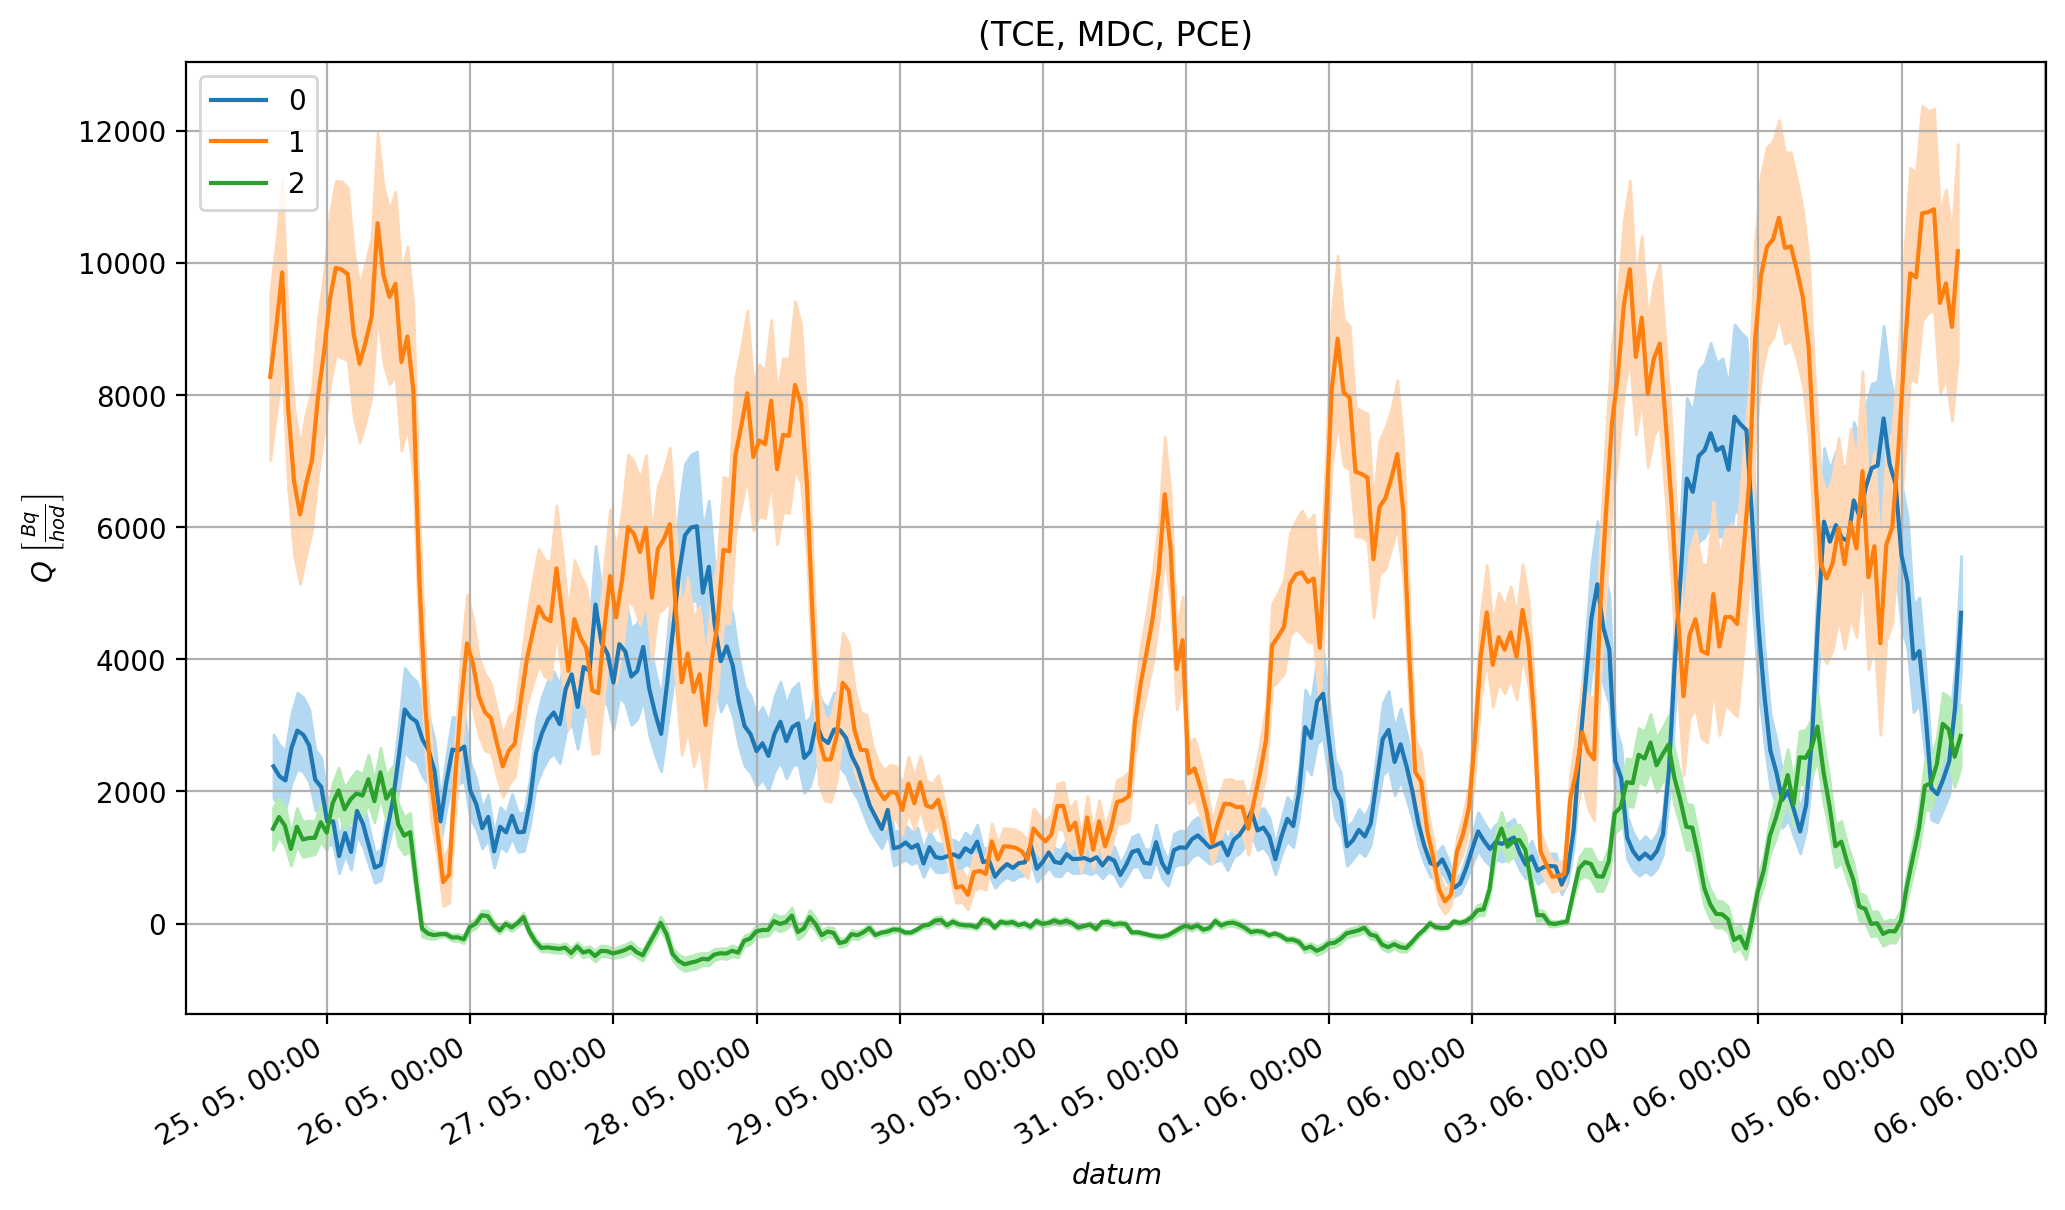
\includegraphics[width=\textwidth]{skala75/prisuny5.png}
    \caption{Určený časový vývoj přísunů radonu do jednotlivých podlaží. Nad obrázkem je uvedena kombinace tří použitých indikačních plynů. Oblasti označené zesvětlenou barvou značí nejistotu přísunů radonu při faktoru pokrytí $k=1$.}
    \label{fig:skala75_prisuny5}
\end{figure}
\begin{table}[H]
    \centering
    \caption{Statistiky vypočítaných přísunů radonu $Q$ do jednotlivých podlaží při stejné kombinaci použitých indikačních plynů jako v obr. nad touto tabulkou.}
    \label{tab:skala75_prisuny5}
    \begin{tabular}{lrrr}
\toprule
{} &  $Q_0$ $\left[\si{\frac{Bq}{m^3\cdot hod}}\right]$ &  $Q_1$ $\left[\si{\frac{Bq}{m^3\cdot hod}}\right]$ &  $Q_2$ $\left[\si{\frac{Bq}{m^3\cdot hod}}\right]$ \\
\midrule
count &                                                284 &                                                284 &                                                284 \\
mean  &                                                113 &                                                250 &                                                 19 \\
%std   &                                                116 &                                                160 &                                                 85 \\
min   &                                                -85 &                                                -78 &                                               -269 \\
25\%   &                                                 37 &                                                111 &                                                -20 \\
50\%   &                                                 74 &                                                255 &                                                 -2 \\
75\%   &                                                161 &                                                369 &                                                 29 \\
max   &                                                528 &                                                913 &                                                371 \\
\bottomrule
\end{tabular}

\end{table}

\begin{figure}[H]
    \centering
    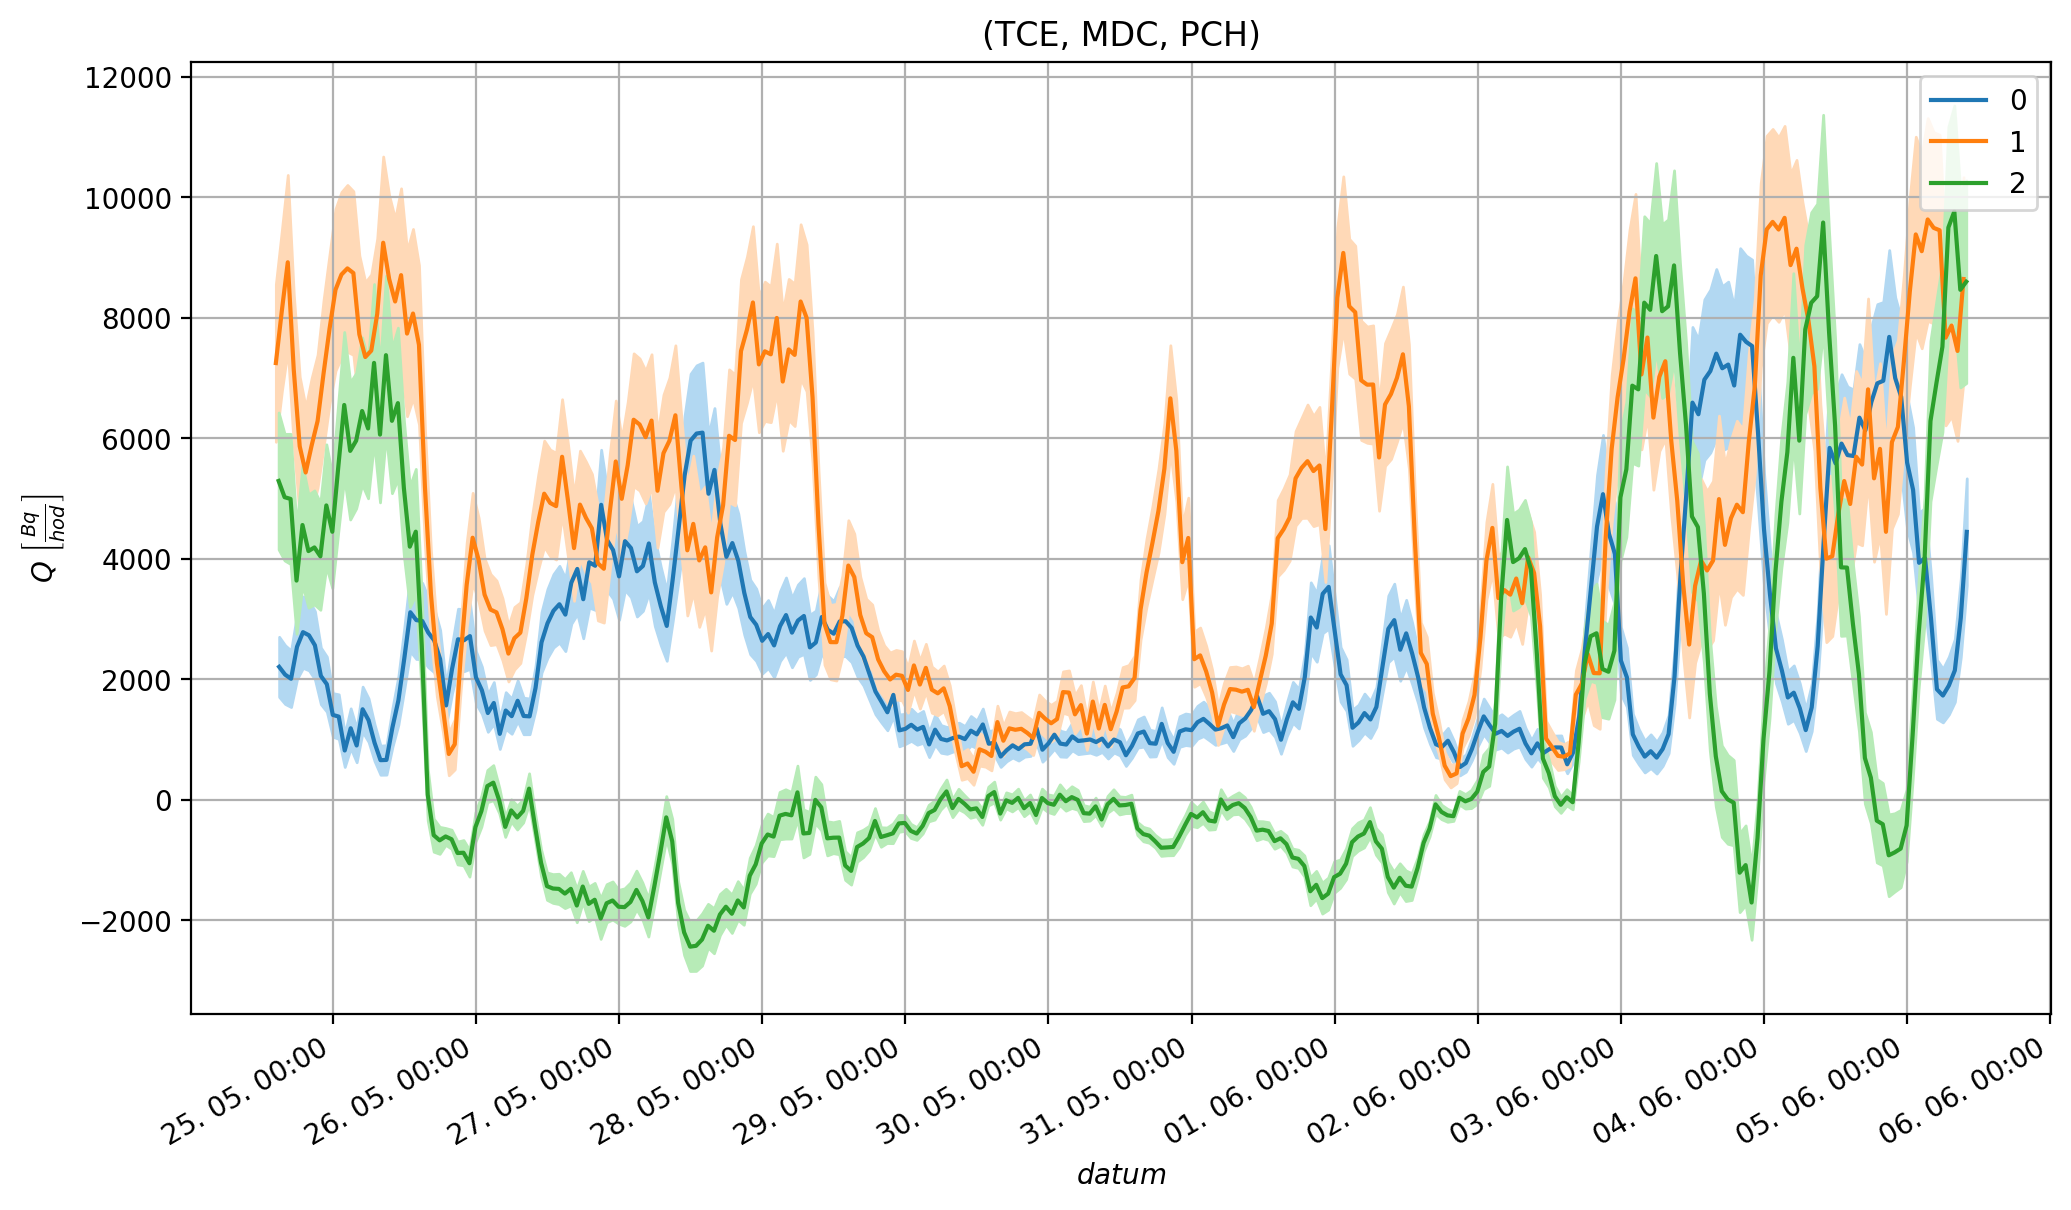
\includegraphics[width=\textwidth]{skala75/prisuny6.png}
    \caption{Určený časový vývoj přísunů radonu do jednotlivých podlaží. Nad obrázkem je uvedena kombinace tří použitých indikačních plynů. Oblasti označené zesvětlenou barvou značí nejistotu přísunů radonu při faktoru pokrytí $k=1$.}
    \label{fig:skala75_prisuny6}
\end{figure}
\begin{table}[H]
    \centering
    \caption{Statistiky vypočítaných přísunů radonu $Q$ do jednotlivých podlaží při stejné kombinaci použitých indikačních plynů jako v obr. nad touto tabulkou.}
    \label{tab:skala75_prisuny6}
    \begin{tabular}{lrrr}
\toprule
{} &  $Q_0$ $\left[\si{\frac{Bq}{hod}}\right]$ &  $Q_1$ $\left[\si{\frac{Bq}{hod}}\right]$ &  $Q_2$ $\left[\si{\frac{Bq}{hod}}\right]$ \\
\midrule
count &                                       284 &                                       284 &                                       284 \\
mean  &                                      4233 &                                     30807 &                                      4359 \\
%std   &                                      4526 &                                     19577 &                                     12339 \\
min   &                                     -4010 &                                    -10346 &                                    -16011 \\
25\%   &                                      1203 &                                     13494 &                                     -3348 \\
50\%   &                                      2855 &                                     31079 &                                      -669 \\
75\%   &                                      6299 &                                     45500 &                                      8645 \\
max   &                                     19350 &                                    110431 &                                     49402 \\
\bottomrule
\end{tabular}

\end{table}

\begin{figure}[H]
    \centering
    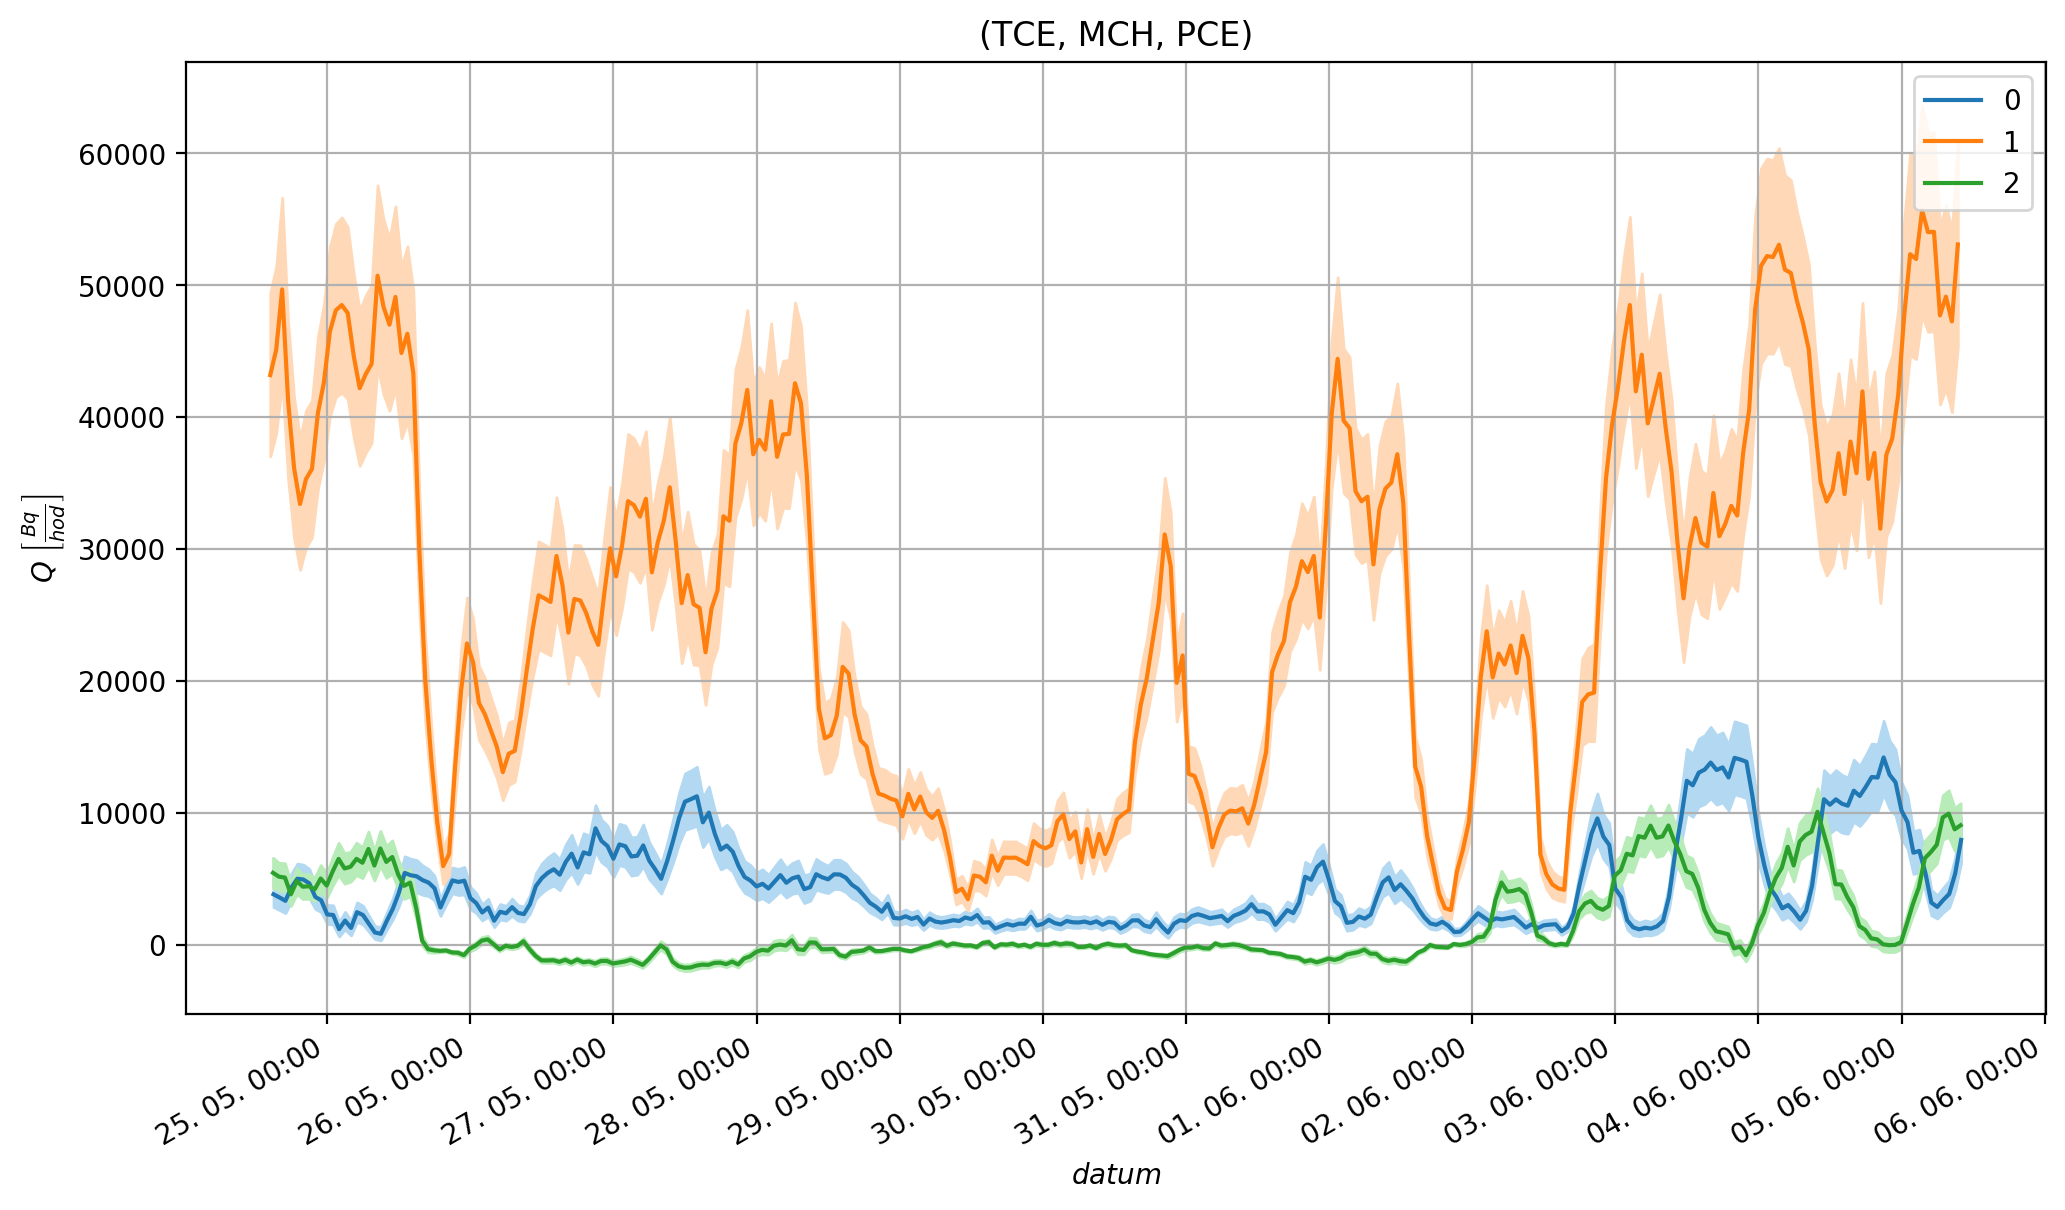
\includegraphics[width=\textwidth]{skala75/prisuny7.png}
    \caption{Určený časový vývoj přísunů radonu do jednotlivých podlaží. Nad obrázkem je uvedena kombinace tří použitých indikačních plynů. Oblasti označené zesvětlenou barvou značí nejistotu přísunů radonu při faktoru pokrytí $k=1$.}
    \label{fig:skala75_prisuny7}
\end{figure}
\begin{table}[H]
    \centering
    \caption{Statistiky vypočítaných přísunů radonu $Q$ do jednotlivých podlaží při stejné kombinaci použitých indikačních plynů jako v obr. nad touto tabulkou.}
    \label{tab:skala75_prisuny7}
    \begin{tabular}{lrrr}
\toprule
{} &  $Q_0$ $\left[\si{\frac{Bq}{hod}}\right]$ &  $Q_1$ $\left[\si{\frac{Bq}{hod}}\right]$ &  $Q_2$ $\left[\si{\frac{Bq}{hod}}\right]$ \\
\midrule
count &                                       284 &                                       284 &                                       284 \\
mean  &                                      4466 &                                     26182 &                                      1325 \\
%std   &                                      3357 &                                     14388 &                                      2973 \\
min   &                                       847 &                                      2646 &                                     -1726 \\
25\%   &                                      1868 &                                     12472 &                                      -540 \\
50\%   &                                      3228 &                                     26241 &                                       -15 \\
75\%   &                                      5735 &                                     37368 &                                      2890 \\
max   &                                     14210 &                                     55660 &                                     10091 \\
\bottomrule
\end{tabular}

\end{table}

\begin{figure}[H]
    \centering
    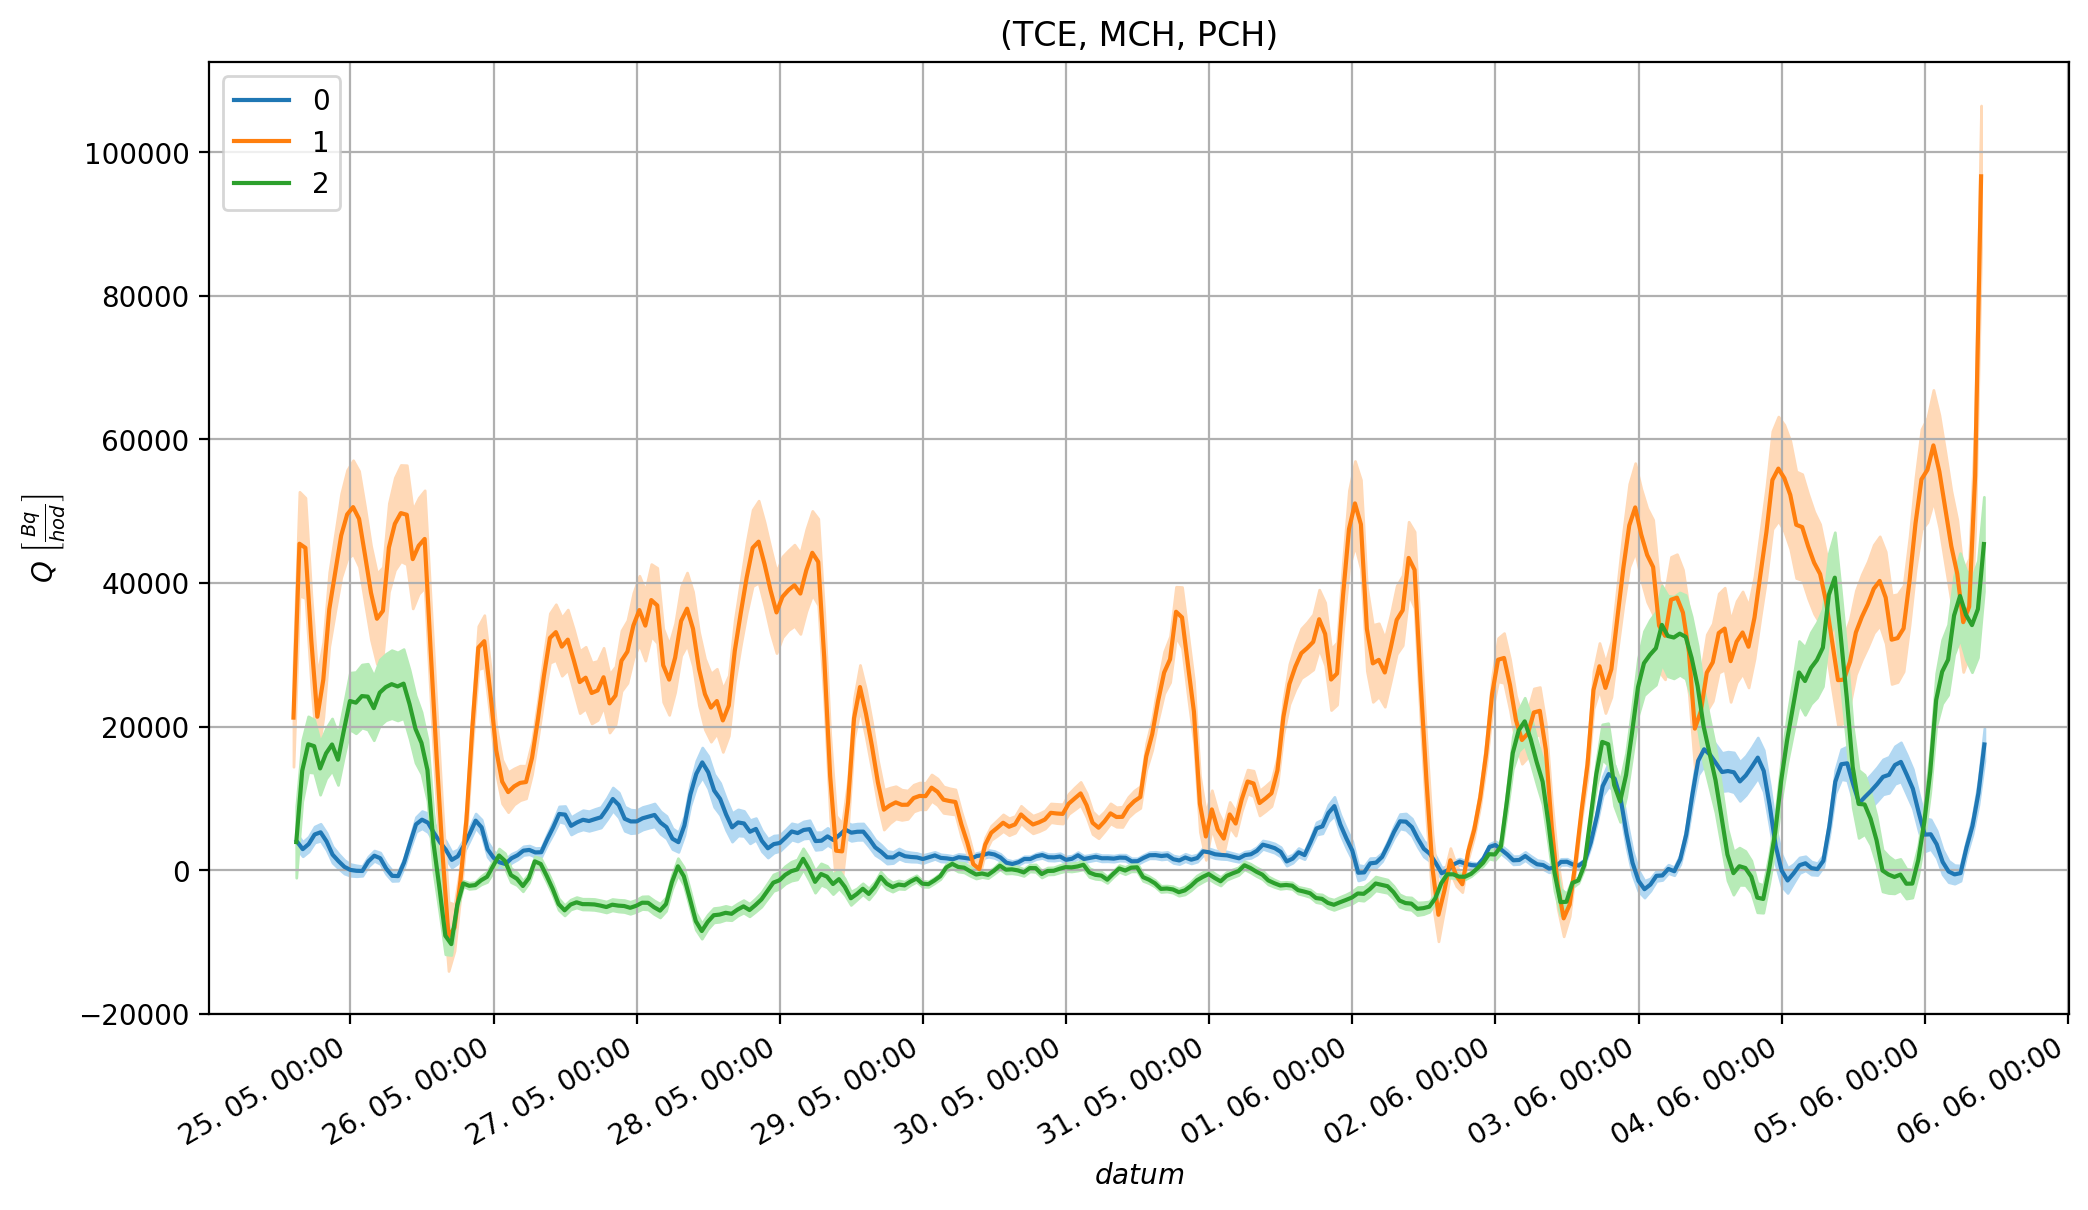
\includegraphics[width=\textwidth]{skala75/prisuny8.png}
    \caption{Určený časový vývoj přísunů radonu do jednotlivých podlaží. Nad obrázkem je uvedena kombinace tří použitých indikačních plynů. Oblasti označené zesvětlenou barvou značí nejistotu přísunů radonu při faktoru pokrytí $k=1$.}
    \label{fig:skala75_prisuny8}
\end{figure}
\begin{table}[H]
    \centering
    \caption{Statistiky vypočítaných přísunů radonu $Q$ do jednotlivých podlaží při stejné kombinaci použitých indikačních plynů jako v obr. nad touto tabulkou.}
    \label{tab:skala75_prisuny8}
    \begin{tabular}{lrrr}
\toprule
{} &  $Q_0$ $\left[\si{\frac{Bq}{m^3\cdot hod}}\right]$ &  $Q_1$ $\left[\si{\frac{Bq}{m^3\cdot hod}}\right]$ &  $Q_2$ $\left[\si{\frac{Bq}{m^3\cdot hod}}\right]$ \\
\midrule
count &                                                284 &                                                284 &                                                284 \\
mean  &                                               2536 &                                               3929 &                                               1148 \\
std   &                                               1795 &                                               2200 &                                               3007 \\
min   &                                                545 &                                                337 &                                              -2379 \\
25\%   &                                               1145 &                                               1866 &                                               -643 \\
50\%   &                                               1934 &                                               3842 &                                               -135 \\
75\%   &                                               3243 &                                               5850 &                                               2588 \\
max   &                                               7736 &                                               8235 &                                               9876 \\
\bottomrule
\end{tabular}

\end{table}

\chapter{Přílohy k objektu Hálková 980, Humpolec}\label{navesti:priloha_humpolec980}

\section{Použitá měřidla}

\begin{itemize}
    \setlength\itemsep{0em}
	\item 20 vyvíječů (4x MDC, 4x MCH, 4x PCE, 4x TCE, 4x TMH)
	\item 8 TD detektorů
	\item 4 CANARY monitory
	\item 4 TERA sondy
	\item 3 TESTO měřiče teploty a vlhkosti
	\item 1 zdroj radonu
\end{itemize}

\section{Naměřené OAR, objemy a teploty}

\begin{table}[H]
    \centering
    \caption{Přiřazení číslování kompartmentů jednotlivým podlažím, objemy všech zón objektu, průměrné teploty naměřené v každém zóně TERA sondami, odhadnuté atmosférické tlaky v každém zóně a průměrné OAR naměřené TERA sondami ($OAR_T$) a CANARY měřáky ($OAR_C$). OAR jsou uvedené v \si{Bq/m^3}.}
    \label{tab:halkova980_objemy}
    \begin{tabular}{lll}
\toprule
podlazi & $OAR$ [\si{Bq/m^3}] & $V$ [\si{m^3}] \\
\midrule
0 &           1094+/-55 &         40+/-8 \\
1 &            562+/-20 &        84+/-10 \\
2 &              51+/-2 &        97+/-15 \\
\bottomrule
\end{tabular}

\end{table}
\begin{figure}[H]
    \centering
    \includegraphics[width=1\textwidth]{halkova980/OAR_dohromady.png}
    \caption{Vývoj OAR naměřený TERA sondami po aplikování kalibračních konstant (tab.~\ref{tab:dynMer_sondyB}).}
    \label{fig:halkova980_OAR_dohromady}
\end{figure}
\begin{figure}[H]
    \centering
    \includegraphics[width=1\textwidth]{halkova980/OAR_CANARY.png}
    \caption{Vývoj OAR naměřený CANARY měřáky.}
    \label{fig:halkova980_OAR_CANARY}
\end{figure}

\section{Objemové průtoky vzduchu}

\begin{table}[H]
    \centering
    \caption{Přehled použitých indikačních plynů a umístění jejich vyvíječů v objektu. V posledním sloupci jsou celkové odpary plynů ze všech jim odpovídajících vyvíječů.}
    \label{tab:halkova980_indikacniPlyny}
    \begin{tabular}{lrrrr}
\toprule
ozn. & podlaží& odpar [mg] &    $M$ [g/mol] &    $U$ $\left[\si{\frac{ng}{ppm\cdot min}}\right]$\\
\midrule
TMH & 0 &192,50 &  450,0 &  8,000 \\
TCE & 0 &193,55 &  130,4 &  1,000 \\
MCH & 1 &472,27 &  350,0 &  8,000 \\
MDC & 1 &497,27 &  400,0 &  8,000 \\
PCH & 2 &230,88 &  450,0 &  8,000 \\
PCE & 2 & 96,54 &  165,8 &  1,385 \\
\bottomrule
\end{tabular}

\end{table}
\begin{table}[H]
    \centering
    \caption{Odezvy TD detektorů $R$ na všechny použité indikační plyny ve všech zónách.}
    \label{tab:halkova980_odezvyTD}
    \begin{tabular}{lrr}
\toprule
plyn & zóna & $R$ [\si{ng}]               \\
\midrule
MCH & 1 & $  36,0\pm2,3$\\
    & 2 & $395,8\pm16,6$\\
    & 3 & $  50,8\pm2,3$\\
MDC & 1 & $  34,5\pm1,2$\\
    & 2 & $ 304,9\pm7,1$\\
    & 3 & $  47,2\pm1,2$\\
TMH & 1 & $145,3\pm26,0$\\
    & 2 & $  37,5\pm3,9$\\
    & 3 & $  20,2\pm2,4$\\
PCH & 1 & $  20,7\pm2,4$\\
    & 2 & $  26,9\pm0,7$\\
    & 3 & $ 182,2\pm4,6$\\
TCE & 1 & $191,8\pm14,5$\\
    & 2 & $  32,2\pm1,4$\\
    & 3 & $  25,0\pm1,2$\\
PCE & 1 & $     0,0\pm0,0$\\
    & 2 & $   2,6\pm0,1$\\
    & 3 & $ 136,9\pm4,1$\\
\bottomrule
\end{tabular}

\end{table}

\begin{table}[H]
    \centering
    \caption{Objemové průtoky vzduchu mezi zónami v \si{m^3/hod} a výměna vzduchu $n$ v \si{hod^{-1}}.}
    \label{tab:halkova980_prutoky}
    \begin{tabular}{l
        >{\collectcell\num}r<{\endcollectcell}
        @{${}\pm{}$}
        >{\collectcell\num}r<{\endcollectcell}
        >{\collectcell\num}r<{\endcollectcell}
        @{${}\pm{}$}
        >{\collectcell\num}r<{\endcollectcell}
}
%\begin{tabular}{l>{\raggedleft\arraybackslash}p{2.5cm}>{\raggedleft\arraybackslash}p{2.5cm}}
\toprule
%{} & (MDC, PCE, TCE, TMH) & (MDC, MCH, TCE, TMH) \\
{} & \multicolumn{2}{r}{(MDC, PCE,} & \multicolumn{2}{r}{(MDC, MCH,} \\
{} & \multicolumn{2}{r}{TCE, TMH)} &   \multicolumn{2}{r}{TCE, TMH)} \\
\midrule
$k_{12}$          &    12,2&4,9 &          40,4&13,4   \\
$k_{13}$          &     4,8&8,9 &           11,9&8,2   \\
$k_{14}$          &   96,0&35,9 &          92,9&34,0   \\
$k_{21}$          &   31,3&27,5 &          40,5&14,8   \\
$k_{23}$          &    17,9&7,9 &            4,4&3,3   \\
$k_{24}$          &   13,8&24,1 &          19,7&12,7   \\
$k_{31}$          &   63,4&26,0 &          62,6&26,1   \\
$k_{32}$          &     1,9&2,8 &            6,2&8,9   \\
$k_{34}$          &   46,9&24,3 &          46,5&23,9   \\
$k_{41}$          &   76,3&37,1 &          74,6&37,7   \\
$k_{42}$          &     4,1&4,1 &          13,6&13,2   \\
$k_{43}$          &    18,0&9,7 &           20,4&9,9   \\
&\multicolumn{2}{r}{}&\multicolumn{2}{r}{}\\
$k_{1_E}$          &   72,6&18,6 &          45,3&11,8   \\
$k_{2_E}$          &  -39,9&15,3 &           12,1&4,6   \\
$k_{3_E}$          &  -27,3&12,3 &          -31,5&8,8   \\
$k_{4_E}$          &   50,9&18,7 &          41,7&13,4   \\
$k_{1_I}$          &   14,7&67,4 &          12,7&62,2   \\
$k_{2_I}$          &    5,0&41,0 &          16,6&29,1   \\
$k_{3_I}$          &   44,2&40,8 &          47,1&39,8   \\
$k_{4_I}$          &   -7,5&65,6 &          -8,8&61,4   \\
\midrule
$n$  &     0,4&0,2 &            0,4&0,1   \\   
\bottomrule
\end{tabular}

    
    
    
    
    
    
    
    
    
    
    
    
    
    
    
    
    
    
    
    
    


\end{table}

\chapter{Přílohy k objektu Anglická 574, Dobřichovice}\label{navesti:priloha_anglicka574}

\section{Fotografie objektu}
\begin{figure}[ht]
    \centering
    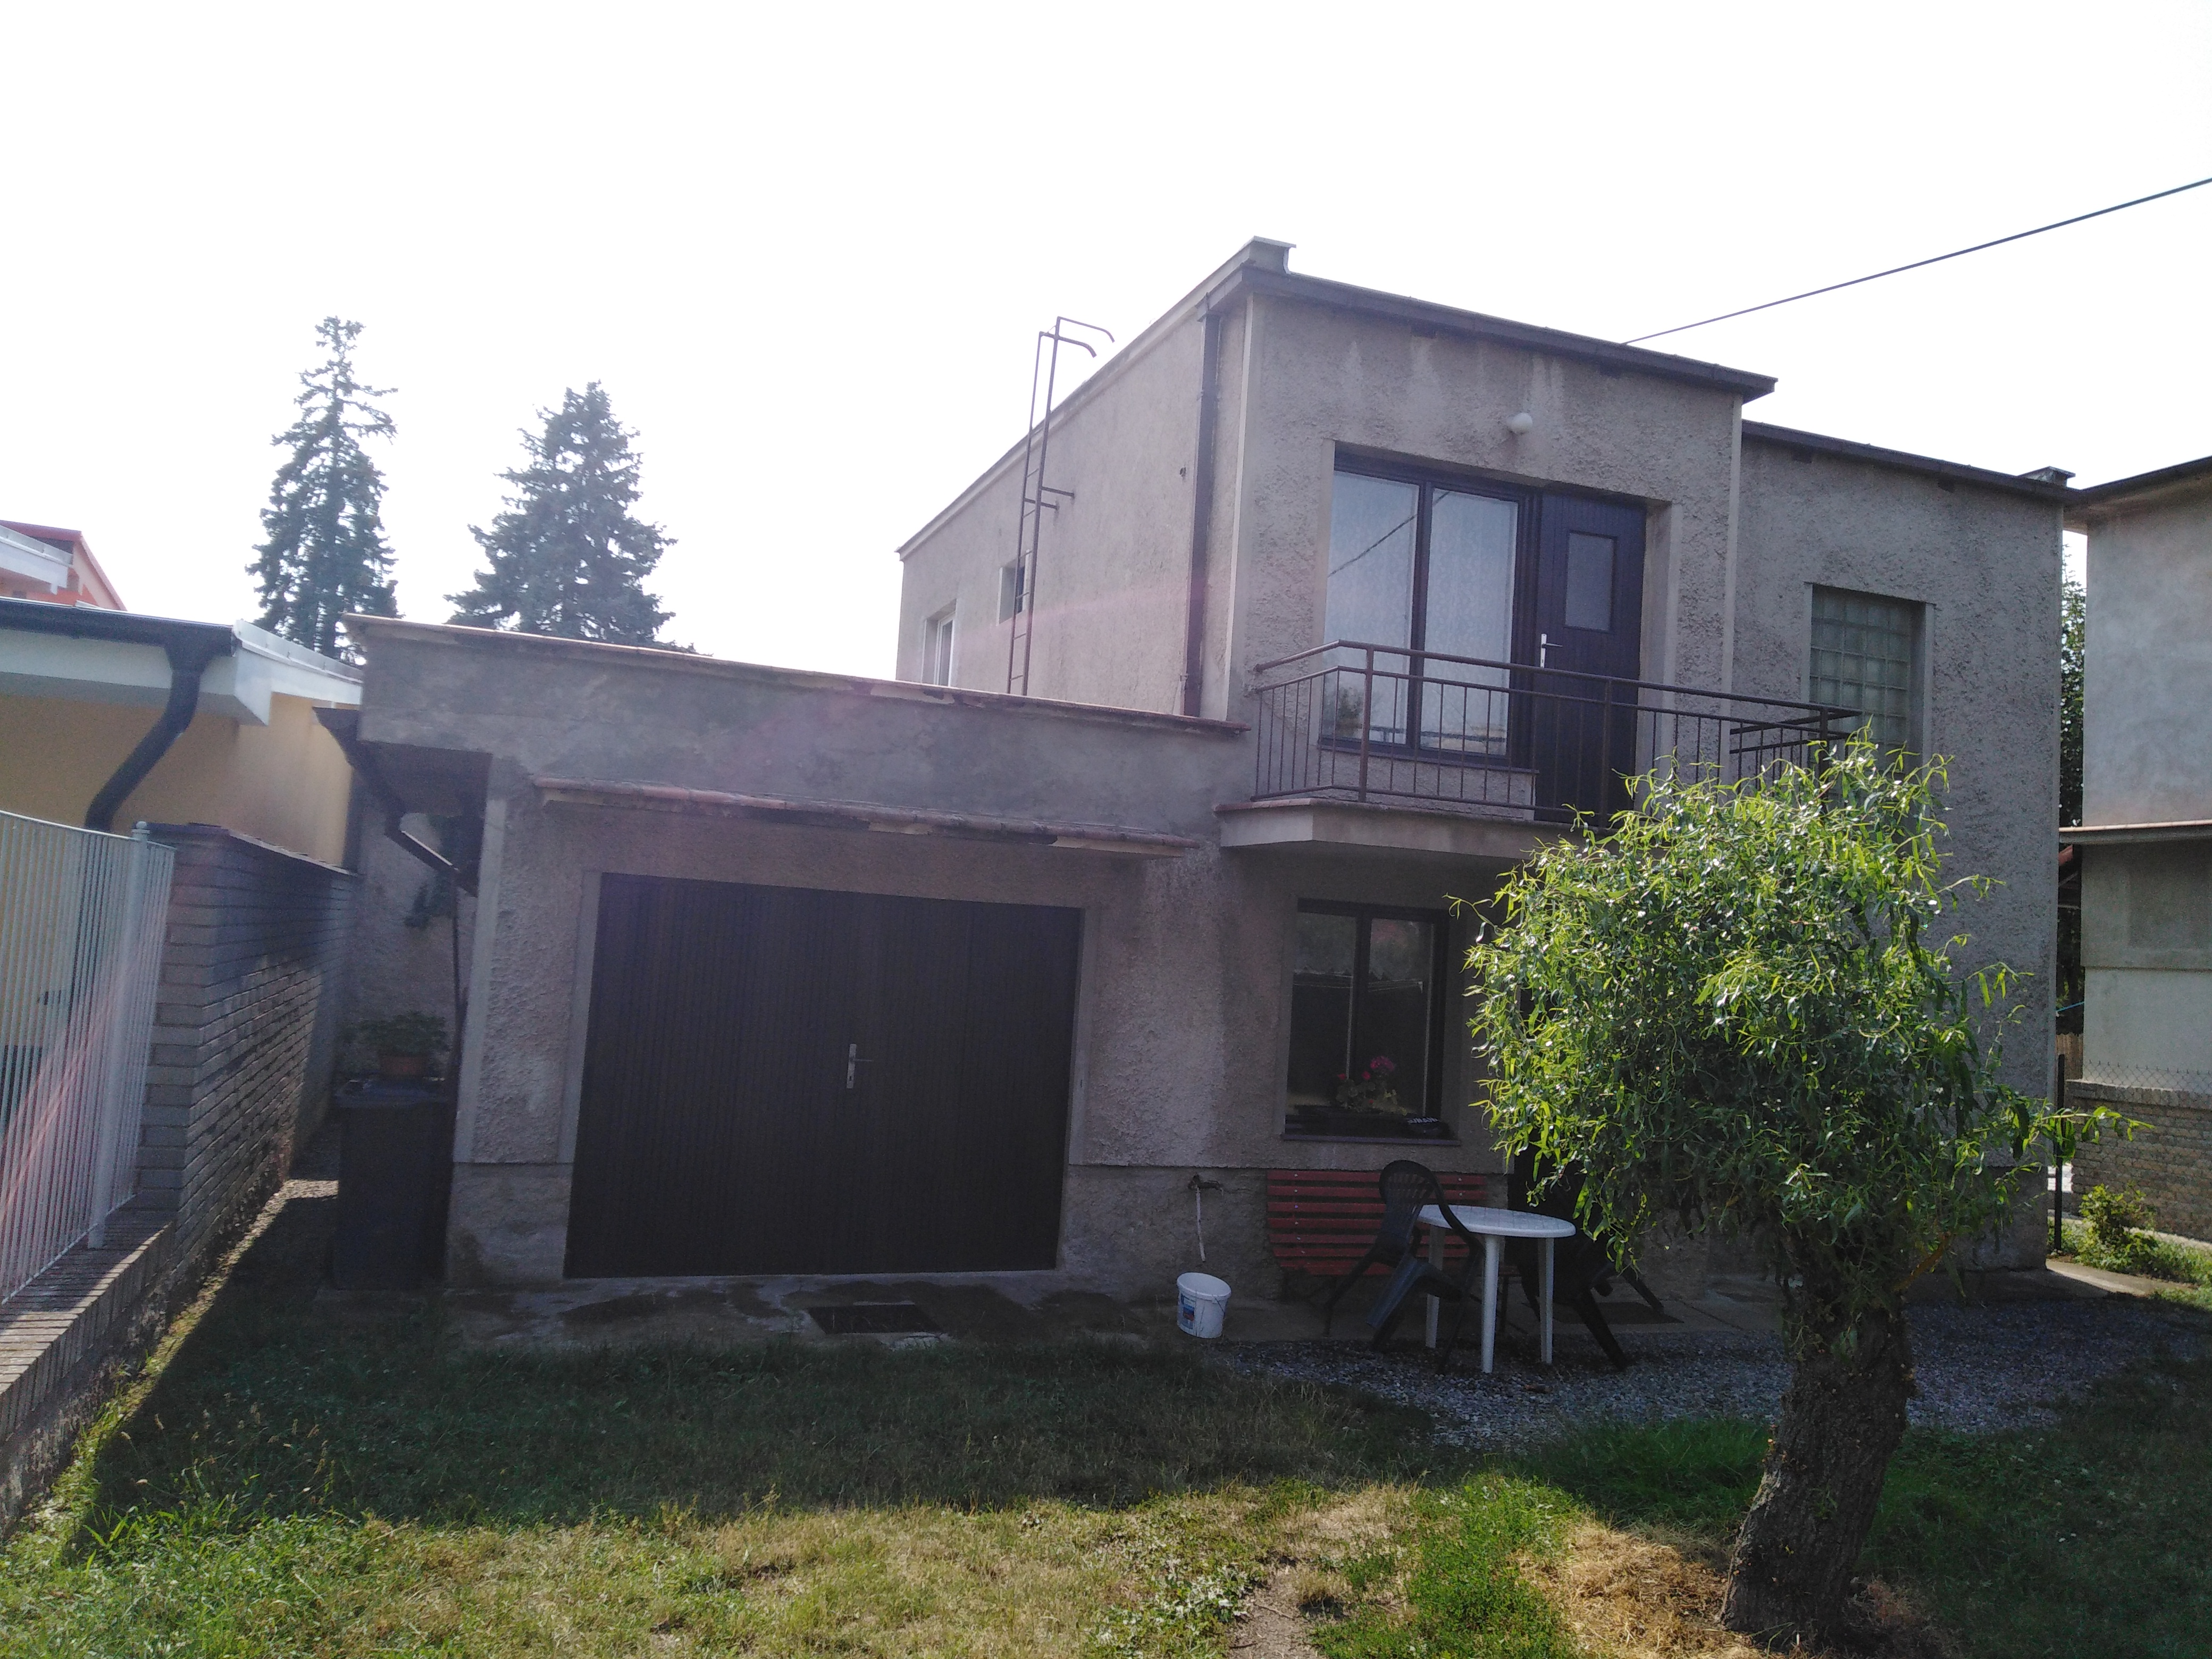
\includegraphics[width=.8\textwidth]{anglicka574/dobrichovice.jpg}
    \caption{Fotografie objektu z přední strany.}
    \label{fig:anglicka574_fotografie}
\end{figure}


\section{Použitá měřidla}
\begin{itemize}
    \setlength\itemsep{0em}
	\item 12 vyvíječů (4x MCH, 4x MDC, 4x PCH)
	\item 12 TD detektorů
	\item 2 blank TD detektory 
	\item 4 CANARY monitory
	\item 4 TERA sondy
	\item 3 TESTO měřiče teploty a vlhkosti
	\item 2 zdroje radonu
\end{itemize}

\section{Naměřené OAR, objemy a teploty}

\begin{table}[H]
    \centering
    \caption{Objemy všech podlaží objektu, průměrné teploty naměřené v každém podlaží TERA sondami, odhadnuté atmosférické tlaky v každém podlaží, průměrné OAR naměřené TERA sondami ($OAR_T$) a CANARY měřáky ($OAR_C$) a přiřazení číslování kompartmentů jednotlivým podlažím. OAR jsou uvedené v \si{Bq/m^3}.}
    \label{tab:anglicka574_objemy}
    \begin{tabular}{lll}
\toprule
podlazi & $OAR$ [\si{Bq/m^3}] & $V$ [\si{m^3}] \\
\midrule
0 &           1094+/-55 &         40+/-8 \\
1 &            562+/-20 &        84+/-10 \\
2 &              51+/-2 &        97+/-15 \\
\bottomrule
\end{tabular}

\end{table}
\begin{figure}[H]
    \centering
    \includegraphics[width=1\textwidth]{anglicka574/OAR_dohromady.png}
    \caption{Vývoj OAR naměřený TERA sondami po aplikování kalibračních konstant (tab.~\ref{tab:dynMer_sondyB}).}
    \label{fig:anglicka574_OAR_dohromady}
\end{figure}
\begin{figure}[H]
    \centering
    \includegraphics[width=1\textwidth]{anglicka574/OAR_CANARY.png}
    \caption{Vývoj OAR naměřený CANARY měřáky.}
    \label{fig:anglicka574_OAR_CANARY}
\end{figure}

\section{Objemové průtoky vzduchu}

\begin{table}[H]
    \centering
    \caption{Přehled použitých indikačních plynů a umístění jejich vyvíječů v objektu. V posledním sloupci jsou celkové odpary plynů ze všech jim odpovídajících vyvíječů.}
    \label{tab:anglicka574_indikacniPlyny}
    \begin{tabular}{lrrrr}
\toprule
ozn. & podlaží& odpar [mg] &    $M$ [g/mol] &    $U$ $\left[\si{\frac{ng}{ppm\cdot min}}\right]$\\
\midrule
TMH & 0 &192,50 &  450,0 &  8,000 \\
TCE & 0 &193,55 &  130,4 &  1,000 \\
MCH & 1 &472,27 &  350,0 &  8,000 \\
MDC & 1 &497,27 &  400,0 &  8,000 \\
PCH & 2 &230,88 &  450,0 &  8,000 \\
PCE & 2 & 96,54 &  165,8 &  1,385 \\
\bottomrule
\end{tabular}

\end{table}
\begin{table}[H]
    \centering
    \caption{Odezvy TD detektorů $R$ na všechny použité indikační plyny ve všech zónách.}
    \label{tab:anglicka574_odezvyTD}
    \begin{tabular}{lrr}
\toprule
plyn & zóna & $R$ [\si{ng}]               \\
\midrule
MCH & 1 & $  36,0\pm2,3$\\
    & 2 & $395,8\pm16,6$\\
    & 3 & $  50,8\pm2,3$\\
MDC & 1 & $  34,5\pm1,2$\\
    & 2 & $ 304,9\pm7,1$\\
    & 3 & $  47,2\pm1,2$\\
TMH & 1 & $145,3\pm26,0$\\
    & 2 & $  37,5\pm3,9$\\
    & 3 & $  20,2\pm2,4$\\
PCH & 1 & $  20,7\pm2,4$\\
    & 2 & $  26,9\pm0,7$\\
    & 3 & $ 182,2\pm4,6$\\
TCE & 1 & $191,8\pm14,5$\\
    & 2 & $  32,2\pm1,4$\\
    & 3 & $  25,0\pm1,2$\\
PCE & 1 & $     0,0\pm0,0$\\
    & 2 & $   2,6\pm0,1$\\
    & 3 & $ 136,9\pm4,1$\\
\bottomrule
\end{tabular}

\end{table}

\begin{table}[H]
    \centering
    \caption{Objemové průtoky vzduchu mezi zónami v \si{m^3/hod} a výměna vzduchu $n$ v \si{hod^{-1}}.}
    \label{tab:anglicka574_prutoky}
    \begin{tabular}{lllll}
\toprule
{} &            0 &          1 &              2 & vnější prostředí \\
\midrule
0                &            0 &  1.3+/-0.4 &  0.033+/-0.029 &           45+/-8 \\
1                &    2.5+/-0.7 &          0 &    0.47+/-0.16 &           23+/-4 \\
2                &  0.14+/-0.12 &  1.3+/-0.4 &              0 &       16.2+/-2.9 \\
vnější prostředí &       44+/-8 &     23+/-4 &     17.1+/-2.9 &                0 \\
\bottomrule
\end{tabular}

\end{table}

\section{Přísuny radonu - grafy a statistiky}
V tomto oddíle jsou uvedeny časové vývoje $Q_i(t)$ z naměřených časových vývojů OAR TERA sondami pro všechny kombinace použitých indikačních plynů.
\begin{figure}[ht]
    \begin{subfigure}{\textwidth}
        \centering
        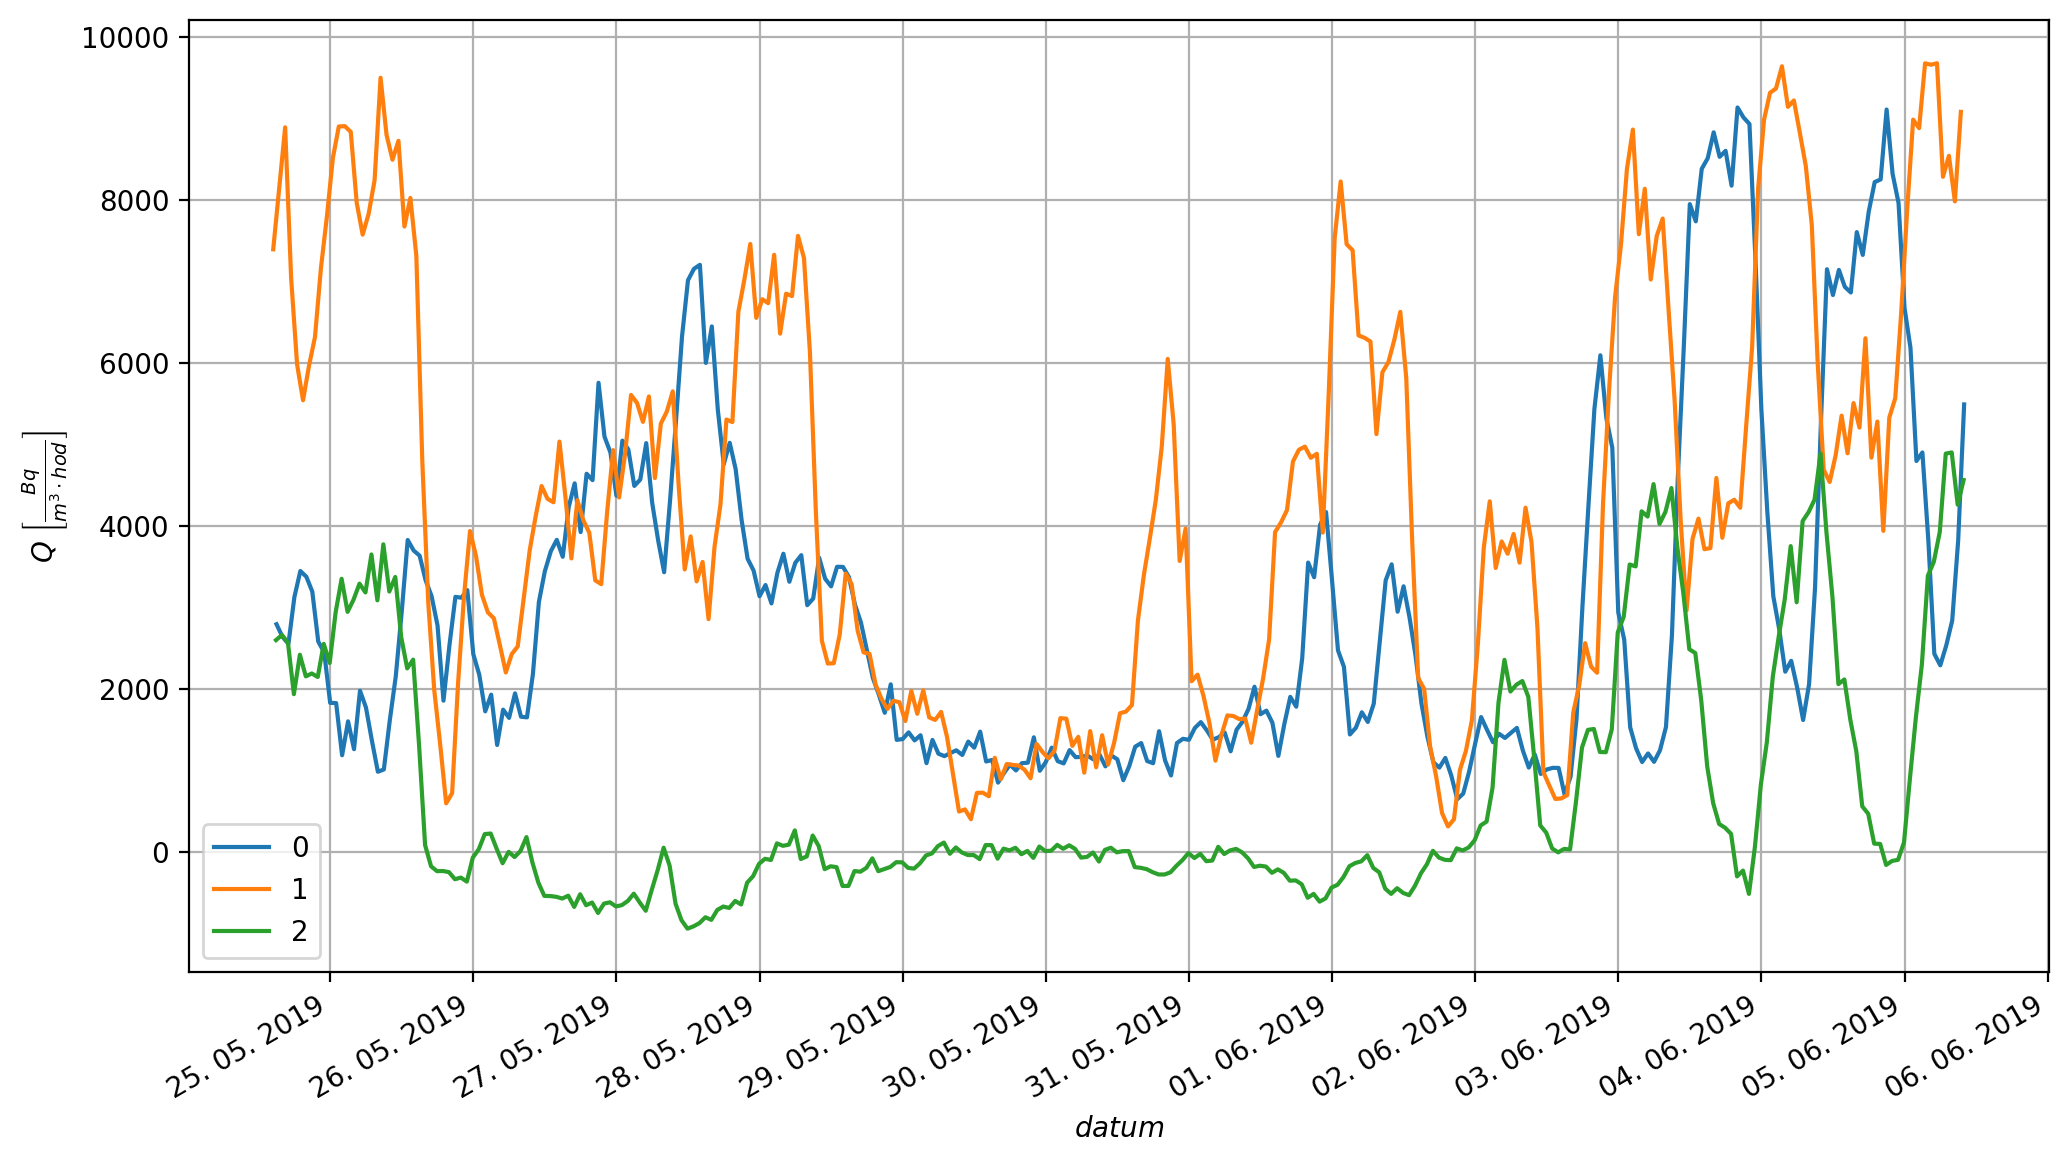
\includegraphics[width=\textwidth]{anglicka574/prisuny.png}
        \caption{}
        \label{fig:anglicka574_prisuny}
    \end{subfigure}
    \begin{subfigure}{\textwidth}
        \centering
        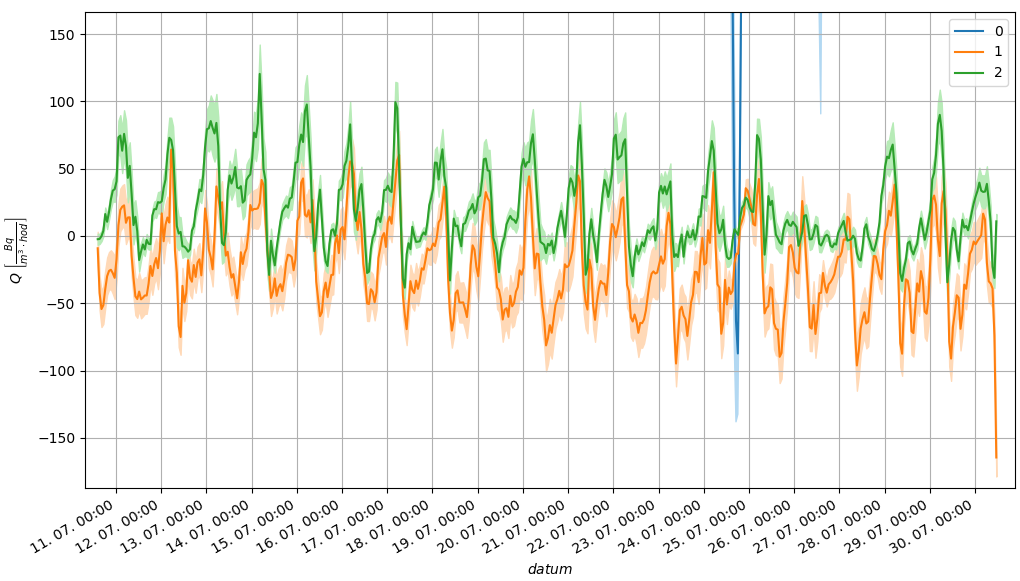
\includegraphics[width=\textwidth]{anglicka574/prisuny_zoom.png}
        \caption{}
        \label{fig:anglicka574_prisunyZoom}
    \end{subfigure}
    \caption{V (a) jsou určené časové vývoje přísunů radonu do jednotlivých podlaží. V (b) jsou přiblížené přísuny radonu do přízemí a prvního patra. Oblasti označené zesvětlenou barvou značí nejistotu přísunů radonu při faktoru pokrytí $k=1$.}
\end{figure}
\begin{table}[H]
    \centering
    \caption{Statistiky vypočítaných přísunů radonu $Q$ do jednotlivých podlaží.}
    \label{tab:anglicka574_prisuny}
    \begin{tabular}{lrrr}
\toprule
{} &  $Q_0$ $\left[\si{\frac{Bq}{m^3\cdot hod}}\right]$ &  $Q_1$ $\left[\si{\frac{Bq}{m^3\cdot hod}}\right]$ &  $Q_2$ $\left[\si{\frac{Bq}{m^3\cdot hod}}\right]$ \\
\midrule
count &                                                284 &                                                284 &                                                284 \\
mean  &  3035 &      4367 &     677 \\
std   &  2122 &      2579 &    1470 \\
min   &                                                652 &                                                319 &                                               -934 \\
25%   &                                               1377 &                                               2000 &                                               -224 \\
50%   &                                               2397 &                                               4104 &                                                 11 \\
75%   &                                               3830 &                                               6310 &                                               1389 \\
max   &                                               9130 &                                               9673 &                                               4902 \\
\bottomrule
\end{tabular}

\end{table}
%\section{Naměřené vývoje OAR, teplot a relativní vlhkosti vzduchu}
%\begin{figure}[ht]
    %\centering
    %\includegraphics[width=1\textwidth]{anglicka574/a1.png}
    %\caption{Data z TERA sondy č. 8, která byla umístěna ve sklepě.}
    %\label{fig:anglicka574_a1}
%\end{figure}
%\begin{figure}[ht]
    %\centering
    %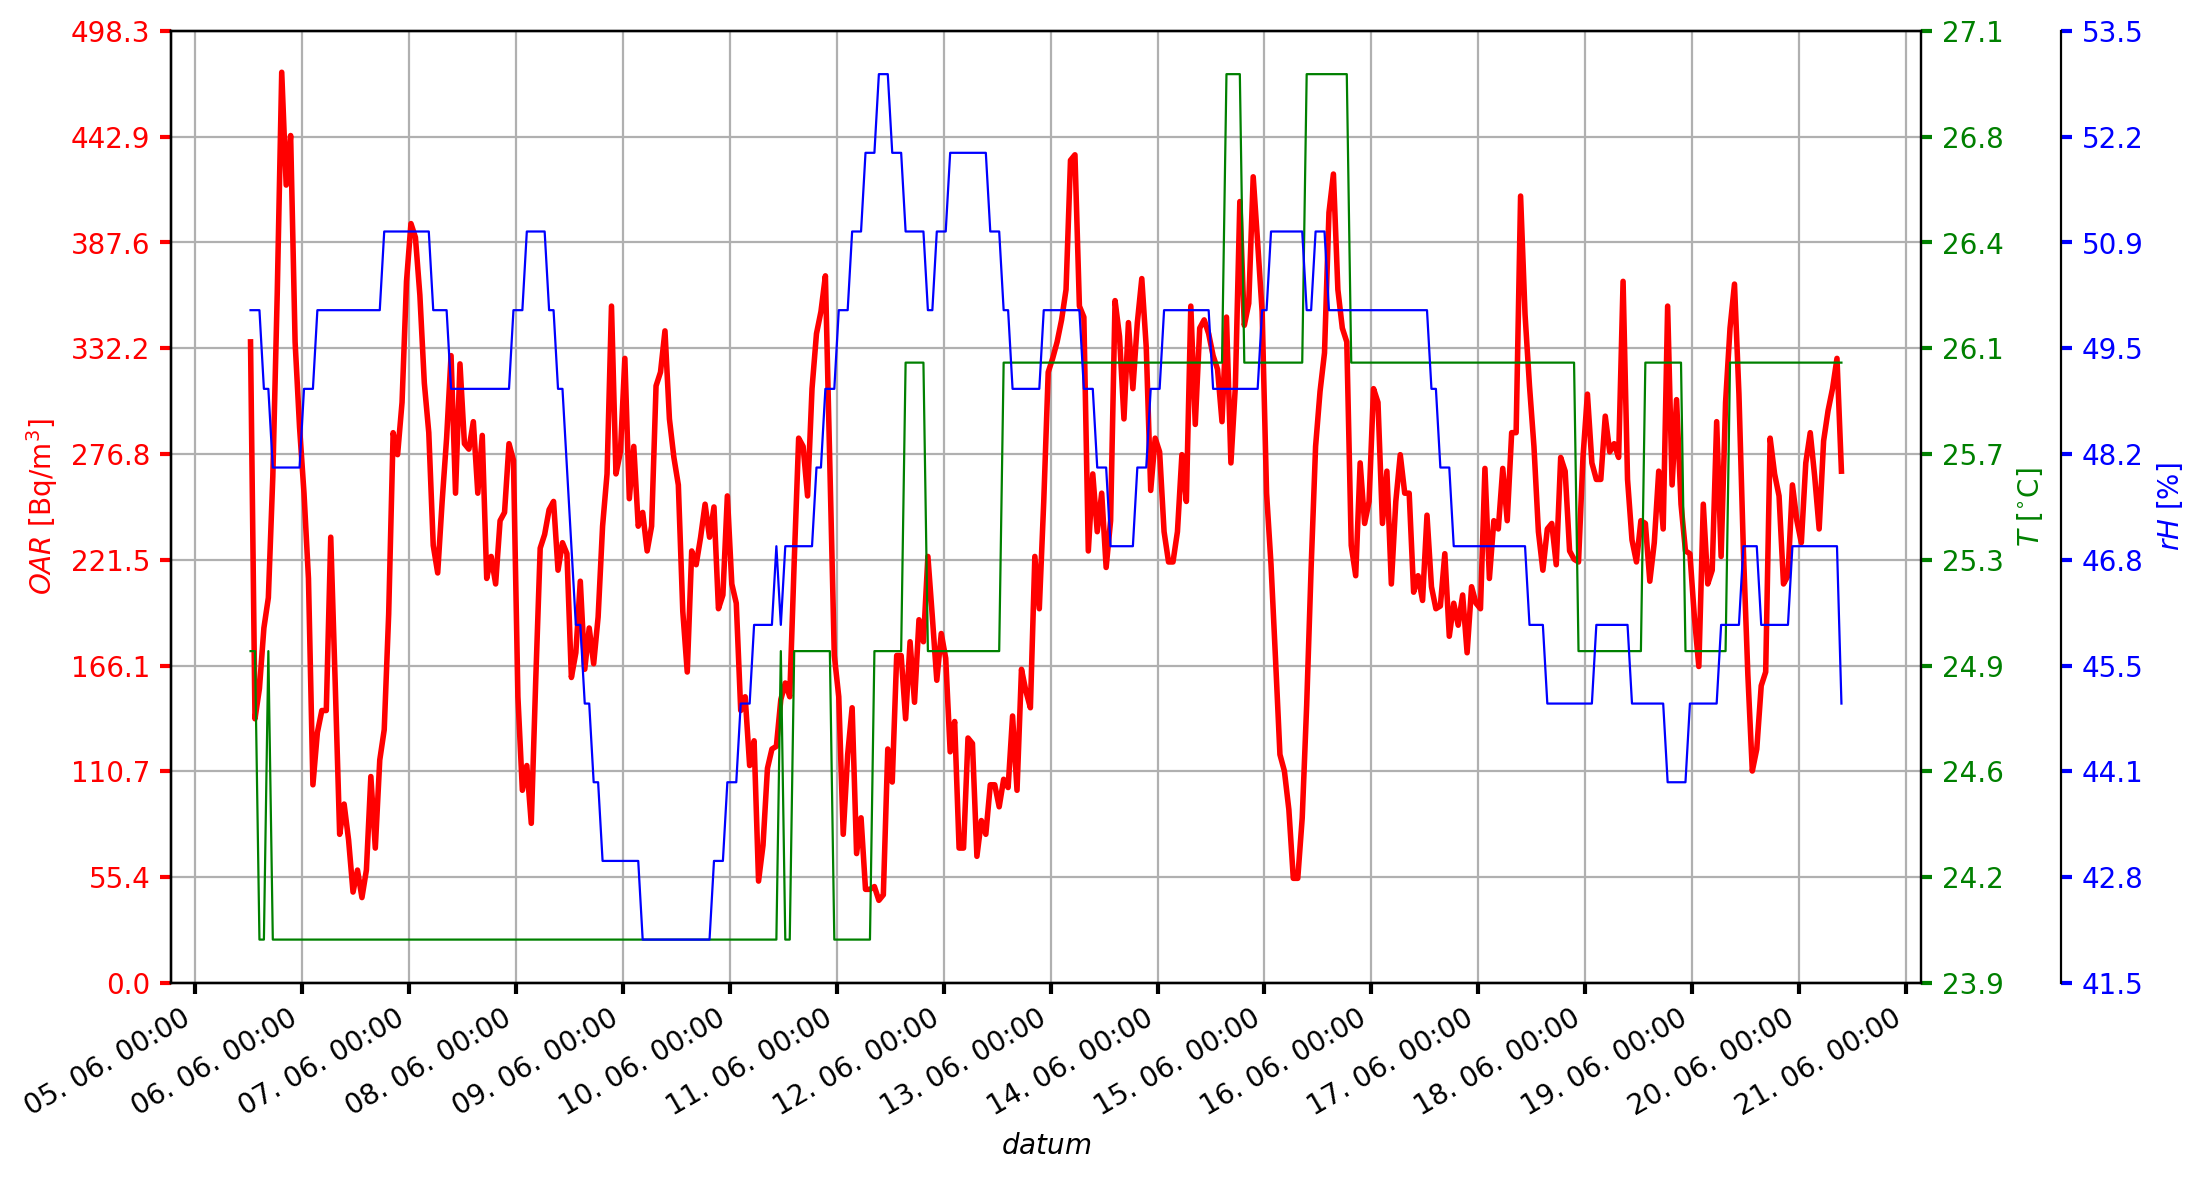
\includegraphics[width=1\textwidth]{anglicka574/a2.png}
    %\caption{Data z TERA sondy č. 88, která byla umístěna v přízemí.}
    %\label{fig:anglicka574_a2}
%\end{figure}
%\begin{figure}[ht]
    %\centering
    %\includegraphics[width=1\textwidth]{anglicka574/a3.png}
    %\caption{Data z TERA sondy č. 112, která byla umístěna v prvním patře.}
    %\label{fig:anglicka574_a3}
%\end{figure}

